\documentclass{article}[14pt]
\usepackage{fancyhdr}
\usepackage{hyperref}
\usepackage{lineno}
\usepackage{graphicx} 
\usepackage{lscape}
\usepackage[pdftex]{thumbpdf}
%\usepackage{draftcopy}
%\usepackage{drafwatermark}
\usepackage{listings}
\usepackage{timestamp}
%%%\usepackage{keyval}
\usepackage[usenames]{color}
\usepackage{type1cm}
\usepackage{eso-pic}

%%%%\usepackage{hyperxmp}
%%\usepackage{tikz}

 \hypersetup{breaklinks=true,
   pdfpagemode=UseOutlines,
   pdffitwindow=true,
   bookmarksopenlevel=3,
   bookmarksnumbered=true
 }

\oddsidemargin 0.0in
\evensidemargin 1.0in
\textwidth 6.5in
%\headheight 1.0in
%\topmargin 0.5in
%\textheight 9.0in


\newenvironment{mlist}{\begin{list}{$\bullet$}{\setlength{\itemsep}{0mm} \setlength{\parsep}{1mm} }}{\end{list}}

\newenvironment{widepar}%
  {\setlength{\rightskip}{-15mm}\addtolength{\rightskip}{15mm}}{\par}

\pagestyle{fancy}
%\setlength{\parindent}{0in}

%\fancyfoot[C]{{\small \sc \copyright 2008 National Research Council Canada \\ \thepage }}  


\definecolor{grey}{rgb}{.9,.9,.9}

%\lstset{pascal}
\lstset{
  basicstyle=\small\ttfamily,
  numbers=none,
  numberstyle=\tiny,numbersep=5pt,
  escapeinside={(*@}{@*)},
  basicstyle=\small, % print whole listing small
  keywordstyle=\bfseries,% underlined bold black keywords
%  commentstyle=\color{white}, % white comments
  stringstyle=\ttfamily, % typewriter type for strings
 showstringspaces=false % no special string spaces
}

\hypersetup{%
pdftitle = {LuSql 1.0$\beta$ User Manual},
pdfsubject = {},
pdfkeywords = {Lucene, SQL, MySQL, indexing},
pdfauthor = {Glen Newton},
pdfcreator = {PDFLatex},
}


\title{LuSql v1.0$\beta$ User Manual}
\author{Glen Newton \\
  {\ttfamily \href{mailto:glen.newton@nrc-cnrc.gc.ca}{glen.newton@nrc-cnrc.gc.ca}\footnote{\url{http://lab.cisti-icist.nrc-cnrc.gc.ca/cistilabswiki/index.php/Glen_Newton}}
}\\
    Canada Institute for Scientific and Technical Information (CISTI)\footnote{\url{http://cisti-icist.nrc-cnrc.gc.ca}}\\
    National Research Council
    Canada\footnote{\url{http://www.nrc-cnrc.gc.ca}}
  }
\date{\today}

%Watermark that works in PDFLates
%  From:
%  http://jeanmartina.blogspot.com/2008/07/latex-goodie-how-to-watermark-things-in.html

%%%% Comment out hte below for draft mode:::
% \makeatletter
% \AddToShipoutPicture{%
% \setlength{\@tempdimb}{.5\paperwidth}%
% \setlength{\@tempdimc}{.5\paperheight}%
% \setlength{\unitlength}{1pt}%
% \put(\strip@pt\@tempdimb,\strip@pt\@tempdimc){%
% \makebox(0,0){\rotatebox{45}{\textcolor[gray]{0.95}%
% {\fontsize{3cm}{3cm}\selectfont{DRAFT}}}}%
% \makebox(-100,-300){\rotatebox{45}{\textcolor[gray]{0.95}%
% {\fontsize{2cm}{2cm}\selectfont{Do not distribute}}}}
% \makebox(-500,-0){\rotatebox{90}{\textcolor[gray]{0.95}%
% {\fontsize{0.7cm}{0.7cm}\selectfont{\timestamp}}}}
% }%
% }
%\makeatother



\begin{document}
\maketitle
\begin{abstract}
LuSql is a simple yet powerful high-performance tool for building Lucene
indexes from relational databases. 
It is a command-line Java application that builds a Lucene 
index from an arbitrary SQL query of a JDBC accessible SQL database.
It allows a user to control a number of parameters, including the
SQL query to use,
individual indexing/storage/term-vector nature of fields, 
analyzer, 
stop word list, 
and other tuning parameters.
In its default mode, it uses threading to take advantage of multiple
cores.
It can handle complex queries, allows for additional per record
sub-queries, and has a plug-in architecture for arbitrary document
manipulation.  
Its only dependencies are the the Lucene core, 
three Apache Commons libraries, 
and a JDBC driver.


%% \Acrobatmenu{Print}{Print}
%% \Acrobatmenu{ZoomIn}{+}
%% \Acrobatmenu{ZoomOut}{-}

\thispagestyle{empty}
\vspace*{5cm}
\begin{center}
{\sc \copyright 2008 National Research Council Canada }

\vspace*{5mm}
  \href{http://creativecommons.org/licenses/by-sa/2.5/ca/}{\includegraphics[width=2cm]{images/creativeCommons.png}}
\end{center}

\end{abstract}
\newpage
\tableofcontents
\newpage
\listoffigures
\newpage
%\linenumbers


\section{Introduction}

LuSql\footnote{LuSql: {\em loo'-skwill}} is an easy to use, high-performance
command-line Java application originally designed to allow users to create
Lucene indexes from the results of a SQL query of a SQL database, but now
extended to be a ZZZZ, allowing data migration from a number of source and
destination platforms using a plug-in architecture.

While LuSql does support JDBC --> Lucene migration directly, it also comes
with a number of drivers for other systems.
These include:
sources:
JDBC, BDB, Java serialized objects
sinks:
JDBC, BDB, XML, text, Lucene, Minion, Solr (via SolrJ), Serialized



\subsection{Why LuSql?}
Many users have their data in a DBMS and some have the need to move
this data to Lucene.
For some, they find that their needs for full-text indexing are not well-met
by their DBMS. 
For others, they need a web facing searchable cache of data stored in their
DBMS.  

Whatever the specific use case, moving this data to Lucene is an effective and
fairly common solution.  
But how to do this?
On the Lucene user mailing
list\footnote{\url{http://mail-archives.apache.org/mod_mbox/lucene-java-user}},
periodically someone asks if there are simple tools for doing this sort of
data transfer:
\begin{lstlisting}[backgroundcolor=\color{grey}]
 To: java-user@lucene.apache.org
 From: "???" <xx.xx.@xxxx.com>
 Subject: Lucene Indexing DB records?
 Date: Fri, 22 Aug 2008 09:26:54 GMT
  
 Guess I don't quite understand why there are so few posts 
 about Lucene indexing DB records. Searched Markmail, but 
 most of the Lucene+DB posts have to do with lucene index 
 management. 
  
 The only thing I found so far is the following, if you 
 have a minute or two:
 http://kalanir.blogspot.com/2008/06/indexing-database-
using-apache-lucene.html
  
 Any comment on this? Efficiency? No need to maintain any 
 intermediate data?
  
 Thanks much,
 -Xxx
\end{lstlisting}


There {\em are} a number of tools which support this sort kind of data transfer
from a DBMS to Lucene, either directly or as part of a larger framework: 
\begin{mlist}
\item SOLR\footnote{\url{http://lucene.apache.org/solr/}}
\item DBSight\footnote{
        \url{http://www.dbsight.net/}
        }
\item Lucene4DB.Net\footnote{
        \url{http://www.netomatix.com/Products/DocumentManagement/Lucene4DB.aspx}
        }
\item Hibernate Search\footnote{
        \url{http://search.hibernate.org/}
        }
\item Compass\footnote{\url{http://www.compass-project.org/}}
\end{mlist}



Without getting into an in-depth analysis of each of these tools, they all suffer
from one or more of the following issues:
\begin{mlist}
\item Overly complicated for non-Lucene / non-Java / non-XML /
  non-framework users
\item Poor performance
\item Not Open Source Software (OSS)
\end{mlist}


LuSql is a simple, high performance, OSS DBMS to Lucene indexing
application that has a very low barrier for use.
Users need the following to use LuSql:
\begin{mlist}
\item Knowledge of SQL
\item Knowledge of their database and tables
\item Ability to set the Java CLASSPATH in a command-line shell
\item Ability to run a command line application
\end{mlist}

At the same time, LuSql offers rich features that make it useful for
some very complex use cases.




\subsection{Features}
LuSql offers control over which
{\tt
    Analyzer}\footnote{\url{http://lucene.apache.org/java/2_3_2/api/org/apache/lucene/analysis/Analyzer.html} 
  }
is applied to the 
{\tt Field}s\footnote{Right now only a single Analyzer is applied to all
  fields. See Section \ref{todo} for more information.} and how/if a
{\tt Field} is stored, indexed, tokenized, compressed, term vectored, etc.

\noindent The SQL query can range from a simple query on a single table: 


\begin{lstlisting}[backgroundcolor=\color{grey}]
  select * from Person;
\end{lstlisting}

\noindent 
to a complex query involving multiple
tables and joins:
%\begin{verbatim}
\begin{lstlisting}[backgroundcolor=\color{grey}]
select Article.id, Article.title, Article.abstract,
 Publisher.name as pub, Journal.title as jo, Journal.issn,
 Volume.number as vol, Volume.coverYear as year, 
 Issue.number as iss from Publisher, Journal, Volume, 
 Issue, Article where Publisher.id =Journal.publisherId and 
 Journal.id = Volume.journalId and Volume.id = Issue.volumeId 
 and Issue.id = Article.issueId;
\end{lstlisting}
%\end{verbatim}

\noindent For extracting additional DBMS information that is difficult or not possible
through a single SQL query, LuSql supports arbitrary per document subqueries.
These subqueries use a field from the original query as a key into other
fields. 

LuSql also offers a plugin architecture for out-of-band
operations on each document {\em after} it is created from the SQL
record but {\em before} it is inserted into the Lucene index. 
An example use case could be where a field in the SQL record is the full path
to a file in the filesystem that contains full-text that the user wants
indexed in a {\tt Field} in addition to the SQL fields already in the document.
 Using the plugin architecture, a Java class can be written and used by LuSql
 to read the file defined by this field and index the contents.



LuSql also offers control over the following:
\begin{mlist}
\item The manner in which specific {\tt Field}s are stored, i.e. index, store,
  and term vector parameters. 
\item Number of documents to add to index from query {\tt ResultSet}
\item Append to or create new Lucene index
\item Stop word list file
\item JDBC URL
\item JDBC driver class\footnote{The default JDBC driver is the MySQL
    driver, {\tt com.mysql.jdbc.Driver}}
\item JDBC {\tt ResultSet} fetch size
\item Lucene RAM buffer size 
\item Number of worker threads; worker queue size
\end{mlist}

\subsubsection{What LuSql is not}
Some of the tools mentioned above offer various features, like automatically
building a web search interface for the created Lucene index.
LuSql only builds a Lucene index.
It is up to the user to decide how they are going to create a user interface
to search the created Lucene index. 


\section{Download and Installation}

\subsection{Download}
The LuSql website
lists\footnote{\url{http://lab.cisti-icist.nrc-cnrc.gc.ca/cistilabswiki/index.php/LuSql}}
  where LuSql bin and src jar files can be downloaded.



\subsection{Dependencies}
LuSql has the following dependencies:
\begin{mlist}
 \item Apache Commons dbcp\footnote{\url{http://commons.apache.org/dbcp/}}. 
   Tested: {\tt commons-dbcp-1.2.2.jar}. 
%   \href{http://cuvier.cisti.nrc.ca/~gnewton/lusql/v0.9/lib/commons-dbcp-1.2.2.jar}{Local copy}

\item Apache Commons cli\footnote{\url{http://commons.apache.org/cli/}}.
   Tested: {\tt commons-cli-1.1.jar}.
%\href{http://cuvier.cisti.nrc.ca/~gnewton/lusql/v0.9/lib/commons-cli-1.1.jar}{Local copy}.

 \item Apache Commons pool\footnote{\url{http://commons.apache.org/pool/}}.
   Tested: {\tt commons-pool-1.4.jar}.
%\href{http://cuvier.cisti.nrc.ca/~gnewton/lusql/v0.9/lib/commons-pool-1.4.jar}{Local copy}.
  
 \item Lucene core\footnote{\url{http://lucene.apache.org/java/docs/releases.html}}.
   Tested: {\tt lucene-core-2.3.1.jar}.
%\href{http://cuvier.cisti.nrc.ca/~gnewton/lusql/v0.9/lib/lucene-core-2.3.1.jar}{Local copy}.

 \item MySQL
     Connector/J JDBC driver\footnote{\url{http://dev.mysql.com/downloads/connector/j/5.1.html}}.
     Tested: {\tt mysql-connector-java-5.0.7-bin.jar}.
%     \href{http://cuvier.cisti.nrc.ca/~gnewton/lusql/v0.9/lib/mysql-connector-java-5.0.7-bin.jar}{Local copy}.
\end{mlist}
\noindent The LuSql jar file contains all of these dependency jar files.

\subsection{Running}
If the versions of these software as included in the LuSql jar file are
appropriate for your use, and the database you wish to connect to is MySQL,
then you can invoke LuSql using the Java {\tt -jar} syntax:
{\small
\begin{lstlisting}[backgroundcolor=\color{grey}]
  java -jar lusql-0.9.jar [command line parameters]
\end{lstlisting}
}

However, if you wish to use a different database driver, a newer version of
Lucene ($>$ 2.3.1) or newer versions of the Apache commons class libraries, you
need to add all of the dependency jars to your {\tt CLASSPATH} and invoke
LuSql in the following manner: 
{\small
\begin{lstlisting}[backgroundcolor=\color{grey}]
  java ca.nrc.cisti.lusql.core.LuSqlMain [command line parameters]
\end{lstlisting}
}

This way of invoking LuSql will NOT use the LuSql dependencies included in the
LuSql jar file, but will instead use the ones in your {\tt CLASSPATH}.



\section{Command Line Arguments}
\begin{description}

\item [\tt -q $<$arg$>$] Primary SQL query (in double quotes). 
  This is passed directly through to the JDBC driver, so non-standard,
  DBMS specific SQL can be used.
  {\bf Required}.


\item[\tt -v] Verbose mode. This prints--out all the parameter values, as well as
  producing a dot (.) for each 1000 records processed, and a running total and
  the time for the previous 10,000 records at each 10,000 records.


\item [\tt -c $<$arg$>$] The JDBC URL to connect to the DBMS. {\bf Required}.

\item [\tt -n $<$arg$>$] Index only the first {\tt n} records from the query.


\item [\tt -l $<$arg$>$] Lucene directory. Default: {\tt ./index}. 


\item [\tt -d $<$arg$>$] Full name of DB driver class (must be in the {\tt
    CLASSPATH}). 
  Default: {\tt com.mysql.jdbc.Driver}


\item [\tt -i $<$arg$>$] LuSql allows control over how each Lucene {\tt Field} is
  indexed.
  This argument allows the user to define the 
  {\tt Field.Index}, {\tt Field.Store} and {\tt Field.TermVector}\footnote{As
    described in
    \url{http://lucene.apache.org/java/2_2_0/api/org/apache/lucene/document/Field.html}.}. 
  The format is "{\tt NNN NNN...NNN}" where each {\tt NNN} triplet corresponds
  to each field returned by the SQL query.
  The three {\tt N}s are integers and indicate the  
  {\tt Field.Index}, {\tt Field.Store} and {\tt Field.TermVector} parameters
  respectively.  
  The values for these integers are shown in Tables 
  \ref{tableIndex}, \ref{tableStore}, \ref{tableVector} in Appendix
  \ref{parameters}. 
  The defaults are {\tt Field.Index.Tokenized}, {\tt Field.Store.YES} and {\tt Field.TermVector.YES}


\item[\tt -I $<$arg$>$] Set all {\tt Field} parameters to be the same with a
  single globel {\tt NNN}. Values as per {\tt -i}.


\item [\tt -g $<$arg$>$] Define a global field=value to be included in {\bf all} {\tt
    Documents} added to the index. 
  Format: "{\tt NNN$|$fieldName=field value}"
  or "{\tt fieldName=field value}". 
  The latter uses the global {\tt -I} setting.
  Multiple {\tt -g} are allowed. {\tt NNN} values as per {\tt -i}.


\item [\tt -t] Test mode. Does not create a Lucene index. 
  Prints (-n) results records from SQL query.


\item [\tt -r $<$arg$>$] Set the RAM buffer size, in MB, of the Lucene {\tt
    IndexWriter}\footnote{\url{http://lucene.apache.org/java/2_3_1/api/org/apache/lucene/index/IndexWriter.html}{setRAMBufferSizeMB(double)}}. 
  Default: 48MB
  (different from Lucene's default of 16MB).
  A larger value will speed-up indexing, at the price of memory usage.


\item [\tt -s $<$arg$>$] Path of stop word file for Lucene to use (relative or full path).


\item [\tt -T]                   Turn off multithreading. Note that multithreading
  does not guarantee the order of documents as retrieved from the DB will
  match their order in the Lucene index.
  If for some reason you need the order of Lucene documents to match the
  order of DB records generated by the SQL query, turn off multithreading.




\item [\tt -N $<$arg$>$] Number of thread for multithreading. Default:\\
  {\tt Runtime.getRuntime().availableProcessors()} *2.5


\item[\tt -Q $<$subquery$>$] Allows for per {\tt Document} SQL subqueries to add additional information
  to the document, using a key field value from the primary query.
  Multiple {\tt -Q} can be used for multiple subqueries.
  See Section \ref{example4} for more information.
  

\item[\tt -A] Append to existing Lucene index (named in {\tt -l}), instead of
  creating anew one (default).


\item[\tt -a $<$class$>$] Full class name implementing Lucene Analyzer. \\
  Default: 
  {\tt org.apache.lucene.analysis.standard.StandardAnalyzer}.


\item[\tt -f $<$arg$>$]   Full class name implementing {\tt DocFilter}. 
  This is applied before each Lucene Document is added to the Index. If it returns null, nothing is added.
  For more information, see Section \ref{filter}.
  Default: {\tt ca.nrc.cisti.lusql.core.NullFilter} (does nothing).


\item [\tt -M $<$arg$>$] Changes the meta replacement string for the {\tt -Q}
 command line parameters. Default: {\tt }@ 


\item [\tt -m]        Turns off the need get around MySQL driver-caused
  OutOfMemory problem in large
  queries\footnote{See
    \url{http://benjchristensen.wordpress.com/2008/05/27/mysql-jdbc-memory-usage-on-large-resultset} for more information}.\\ 
  Sets
  {\tt Statement.setFetchSize(int)}\footnote{\url{http://java.sun.com/j2se/1.5.0/docs/api/java/sql/Statement.html}{setFetchSize(int)}} 
  to {\tt Integer.MIN\_VALUE}.


\item[\tt -p $<$arg$>$] Properties file




\end{description}

\section{Tutorial}
\label{tutorial}

\subsection{Quickstart}
{\small
\begin{lstlisting}[backgroundcolor=\color{grey},language=SQL]
java -jar lusql.jar -l quickstartIndex -q "select * from mytable" \
 -c "jdbc:mysql://dbhost/db?user=ID\&password=PASS"
\end{lstlisting}
}

Create a Lucene index called {\tt quickstartIndex} which indexes all the
fields of all the records in table {\tt mytable}, from database {\tt db}
on MySQL database host {\tt dbhost}, with user {\tt ID}, password {\tt PASS}. 



\subsection{Tutorial-by-example}

This tutorial uses four examples of progressively increasing complexity,
to present different aspects of LuSql functionality.
\begin{mlist}
\item In the first, a single table is queried using a simple SQL query to produce an
index.
\item In the second, a complex set of tables is queried with a join intensive SQL
query.
\item In the third, the second example is extended using per-record
subqueries, to include data from M:N tables.
\item In the fourth, the third example is extended using a {\tt
  DocFilter},
  and uses a field which contains the file system path to a text file whose
  full-text is read and indexed as an additional field.
\end{mlist}

The tutorial assumes a MySQL database, a Linux/Unix--like command-line
  environment, and uses 
  {\bf Luke}\footnote{\url{http://www.getopt.org/luke/}
}
or the {\em Lucene Index Toolbox} to validate the created indexes.
Luke is a Java application that allows - among many other useful things - the 
examination of Lucene indexes and the perusal of the {\tt Document}s and
  {\tt Field}s that the indexes contain.

A description of the hardware, operating system, Java versions, etc. used in
the tutorial can be found in \mbox{Appendix \ref{hardware}}.


\subsection{Example 1: Single table}
\label{example1}
Given the following table:
{\small
\begin{verbatim}
   mysql> describe Article;
   +--------------+-------------+------+-----+---------+-------+
   | Field        | Type        | Null | Key | Default | Extra |
   +--------------+-------------+------+-----+---------+-------+
   | id           | int(11)     | YES  |     | NULL    |       | 
   | articleTitle | varchar(64) | YES  |     | NULL    |       | 
   | abstract     | text        | YES  |     | NULL    |       | 
   | startPage    | varchar(16) | YES  |     | NULL    |       | 
   | journalTitle | text        | YES  |     | NULL    |       | 
   | issn         | char(12)    | YES  |     | NULL    |       | 
   | volumeNumber | varchar(32) | YES  |     | NULL    |       | 
   | volumeYear   | char(16)    | YES  | MUL | NULL    |       | 
   | issueNumber  | varchar(32) | YES  |     | NULL    |       | 
   +--------------+-------------+------+-----+---------+-------+
\end{verbatim}
   
\begin{verbatim}
   mysql> select count(id) from Article;
   select count(id) from Article;
   +-----------+
   | count(id) |
   +-----------+
   |   6409484 | 
   +-----------+
\end{verbatim}

\begin{verbatim}
   mysql> select count(id)  from Article where volumeYear > 2007;
   +-----------+
   | count(id) |
   +-----------+
   |       218 | 
   +-----------+
\end{verbatim}
}

Let's say we want to create a Lucene index, using the
{\tt StandardAnalyzer\footnote{
    \url{http://lucene.apache.org/java/2_3_1/api/org/apache/lucene/analysis/standard/StandardAnalyzer.html}
  }}, 
  and want all fields to be:
\begin{mlist}
\item
{\tt
        Field.Index.TOKENIZED\footnote{\url{http://lucene.apache.org/java/2_3_2/api/org/apache/lucene/document/Field.Index.html}{TOKENIZED}}
}

\item
{\tt
        Field.Store.YES\footnote{\url{http://lucene.apache.org/java/2_3_2/api/org/apache/lucene/document/Field.Store.html}{YES}}
}

\item {\tt Field.TermVector.YES\footnote{\url{http://lucene.apache.org/java/2_3_2/api/org/apache/lucene/document/Field.TermVector.html}{YES}
}
}
\end{mlist}

\noindent but we only want the records that have {\tt volumeYear} $>$  2007 and we
only want the first 100 records.

LuSql offers a ``test'' mode which does no indexing and does not create a Lucene
index, but instead prints the results of your SQL query.
This is to validate that your SQL query is valid, and for you to see if the
fields and their values returned by your query make sense.


Here is how you would invoke LuSql, assuming a Linux shell (bash)
 environment\footnote{In most Unix/Linux shell environments, the
 backslash ($\backslash$) denotes that the command is continued on the
 next line}:

{\small
\begin{lstlisting}[backgroundcolor=\color{grey},language=SQL,numbers=left]
java -jar lusql.jar  \(*@\label{java}@*)
 -q "select * from Article where  volumeYear >  2007" \(*@\label{q}@*)
 -c "jdbc:mysql://dbhost/db?user=ID&password=PASS"\ (*@\label{c}@*)
 -n  5  \(*@\label{n}@*)
 -l tutorial-1 \(*@\label{l}@*)
 -v \(*@\label{v}@*)
 -I 211 \(*@\label{I}@*)
 -t(*@\label{t}@*)
\end{lstlisting}
}



Explanation:
\begin{mlist}
  \item Line \ref{java}: invoke LuSql.
  \item Line \ref{q}: {\tt -q} SQL statement to be used.
  \item Line \ref{c}: {\tt -c} JDBC URL to use.
    Note that this may be different across different JDBC drivers.
  \item Line \ref{c}: {\tt -n} limit the number of records indexed, or, in
    this case ({\tt -t}) the number of records to print out.
  \item Line \ref{l}: {\tt -l} the directory for the Lucene index.
    If the directory does not exist, it will be created.
    If it exists, it will be overwritten (default).
  \item Line \ref{v}: {\tt -v} verbose output showing various attributes and
    a progress indicator.
    The default mode is to produce no console output.
  \item Line \ref{I}: {\tt -I} defines a single set of
    {\tt Field.Index}, {\tt Field.Store}, and {\tt Field.TermVector} values to
    be applied to all fields to be included in the Lucene {\tt Document}. 
    The {\tt -I} parameter has the form {\tt NNN} where the respective {\tt
      Field} attributes are defined as:\label{nnn}
{\small
\begin{verbatim}
       Index: Default:TOKENIZED (2)
        0:NO
        1:NO_NORMS
        2:TOKENIZED
        3:UN_TOKENIZED
       Store: Default:YES (1)
        0:NO
        1:YES
        2:COMPRESS
       Term vector: Default:YES (1)
        0:NO
        1:YES
        2:WITH_OFFSETS
        3:WITH_POSITIONS
        4:WITH_POSITIONS_OFFSETS
\end{verbatim}
}

Note that if neither {\tt -I} nor {\tt -i} is set, the default is: {\tt -I
  211}.  
  \item Line \ref{t}: {\tt -t} test mode
\end{mlist}

Example test ({\tt -t}) output for only 5 records\footnote{Appendix
  \ref{hardware} shows the test configuration for the indexing and DBMS
  hardware} (long lines are truncated with {\tt ...}):
{\small
%\begin{verbatim}
\begin{lstlisting}[backgroundcolor=\color{grey}]
> java -jar lusql.jar -q "select * from Article where volumeYear > 2007" \
  -c "jdbc:mysql://dbhost/db?user=USERID&password=PASSWORD"\
  -n 5 -l tutorial-1 -v -I 211 -t
Using sql:[select * from Article where volumeYear > 2007]
Using Analyzer:[org.apache.lucene.analysis.standard.StandardAnalyzer]
Using Stop Word FileName:[null]
Using Properties FileName:[null]                                                            
Using DB driver name:[com.mysql.jdbc.Driver]
Using DB URL:[jdbc:mysql://dbhost/db?user=USERID\&password=PASSWORD]
Using Lucene index:tutorial-1
Using Lucene index RAMBUFFER MBs:48.0 
Using multithreaded:true  
Using Test:true 
Using Field parameters:211
Using setting DB fetchsize=0 (see -m)
Using Num documents to add:5 
Using Lucene index directory:tutorial-1   
Opening Lucene index: tutorial-1
Opening MySQL connection 
Querying:select * from Article where volumeYear > 2007 
Test only: not indexing: SQL results  
> id=2486095; articleTitle=Complexation of io...; ...
> id=2486107; articleTitle=Microwave-assisted...; ...
> id=2486111; articleTitle=Diffraction effici...; ...
> id=2486116; articleTitle=The synthesis and...; ...
> id=2486119; articleTitle=Synthesis and phot...; ...
Closing JDBC: result set
Closing JDBC: statement
Closing JDBC: connection
*********** Elapsed time: 0 seconds 
\end{lstlisting}
%\end{verbatim}
}
\noindent Perusing the SQL query shows us that this is indeed what we want, so now we
invoke LuSql without the {\tt -t} test flag, and change the number of result
records to index from 5 to 100:
{\small 
%\begin{verbatim}
\begin{lstlisting}[backgroundcolor=\color{grey}]
> java -jar lusql.jar \
-q "select * from Article where volumeYear > 2007"\
-c "jdbc:mysql://dbhost/db?user=USERID&password=PASSWORD"\
-n 100 -l tutorial-1 -v -I 211
Using sql:[select * from Article where volumeYear > 2007]
Using Analyzer:[org.apache.lucene.analysis.standard.StandardAnalyzer]
Using Stop Word FileName:[null]
Using Properties FileName:[null]
Using DB driver name:[com.mysql.jdbc.Driver]
Using DB URL:[jdbc:mysql://dbhost/db?user=USERID&password=PASSWORD]
Using Lucene index:tutorial-1
Using Lucene index RAMBUFFER MBs:48.0
Using multithreaded:true
Using Test:false
Using Field parameters:211
Using setting DB fetchsize=0 (see -m)
Using Num documents to add:100
Using Lucene index directory:tutorial-1
Opening Lucene index: tutorial-1
Opening MySQL connection
Querying:select * from Article where volumeYear > 2007
Indexing
Threading: Queue size=60
Threading: # threads=20

Number of records added= 100

Optimizing index
  Closing index
  Optimizing index time: 0 seconds
Closing JDBC: result set
Closing JDBC: statement
Closing JDBC: connection
*********** Elapsed time: 7 seconds
>
\end{lstlisting}
%\end{verbatim}
}


%% As shown in the output, a number of parameters have implicit default
%% values.
%% We will examine some of these in the more advanced examples, as well
%% examining all command line arguments in Section \ref{cli}.

\subsubsection{Example 1 examined in Luke}
Here, we will use Luke to verify the index we just created.
\begin{mlist}

\item Figure \ref{luke_1_1} shows the index in the Luke {\tt Overview} panel.
  It shows the name of the index, the number of documents, the number of
  documents per field, etc.
  The number of documents, fields, etc., appear to be what we wanted.

\item Figure \ref{luke_1_2} shows the Luke {\tt Documents} panel, which allows for
  the perusal of individual documents and their fields.
  This is used to validate that the right records are in the index, and to check
  exactly how each field has been indexed.
  Hand checking this information with a query of the database validates
  that it is the right information.
  The {\tt Flags} indicating the Lucene storage parameters also appear to be
  what we expect. 

\item Figure \ref{luke_1_3} shows the Luke {\tt Search} panel which allows the user to
  formulate queries and apply them to the index.
  Note that the {\tt Analyzer} selected is the {\tt StandardAnalyzer}\footnote{\tt
    org.apache.lucene.analysis.standard.StandardAnalyzer} which matches the
  one we used in our indexing; the default
  {\tt Analyzer} for Luke is {\tt
    SimpleAnalyzer}\footnote{{\tt org.apache.lucene.analysis.standard.SimpleAnalyzer}}. 
  Using a different {\tt Analyzer} for indexing and querying may result in
  unpredictable (and undesirable) behaviour.
  The query returns the correct, and the correct number of, {\tt Documents}.
  Here is a validating\footnote{
    Caution must be applied when doing this kind of validation, as 
    differences in indexing in Lucene and the SQL database can cause
    significant differences in the type and number of results returned. 
    There is no 1:1 mapping of Lucene queries to SQL queries.
    That said, it is still useful to do this kind of validation querying,
    as long as you understand the results.}
  SQL query:\\
{\small 
\begin{lstlisting}[backgroundcolor=\color{grey}]
  mysql> select id from Article where volumeYear > 2007  \
     and abstract like "%ionic%" and journalTitle like "%pigments%"\
     and articleTitle like "%surfactants%";
   +---------+
   | id      |
   +---------+
   | 2486095 | 
   | 2486179 | 
   +---------+
\end{lstlisting}
}
    While this seems like a problem as the SQL query produces more results
    than Luke (id=2486095 matches what Luke tells us, but id=2486179 does
    not), deeper examination shows that the second id is the $110^th$ record
    returned by {\tt select count(id)  from Article where volumeYear > 2007},
    so it is not in our Lucene index, explaining why Luke does not show it.
\end{mlist}

%\begin{landscape}
  \begin{figure}
  \begin{center}
 \includegraphics[width=\textwidth]{images/luke_1_1.png}
 % \includegraphics[height=\textwidth]{images/luke_1_1.png}
%  \includegraphics[width=16cm]{images/luke_1_1.png}
      \end{center}
  \caption{Example 1 in {\tt Luke}: Overview panel}
\label{luke_1_1}
\end{figure}

%\begin{landscape}
\begin{figure}
  \begin{center}
  % \scalebox{0.5}{
  %\includegraphics[height=\textwidth]{images/luke_1_2.png}
  \includegraphics[width=\textwidth]{images/luke_1_2.png}
        % }
      \end{center}
  \caption{Example 1 in {\tt Luke}: Documents panel}
\label{luke_1_2}
\end{figure}

\begin{figure}
  \begin{center}
%    \includegraphics[height=\textwidth]{images/luke_1_3.png}
    \includegraphics[width=\textwidth]{images/luke_1_3.png}
  \end{center}
  \caption{Example 1 in {\tt Luke}: Search panel}
  \label{luke_1_3}
\end{figure}
%\end{landscape}


\begin{landscape}
\begin{figure}
  \begin{center}
    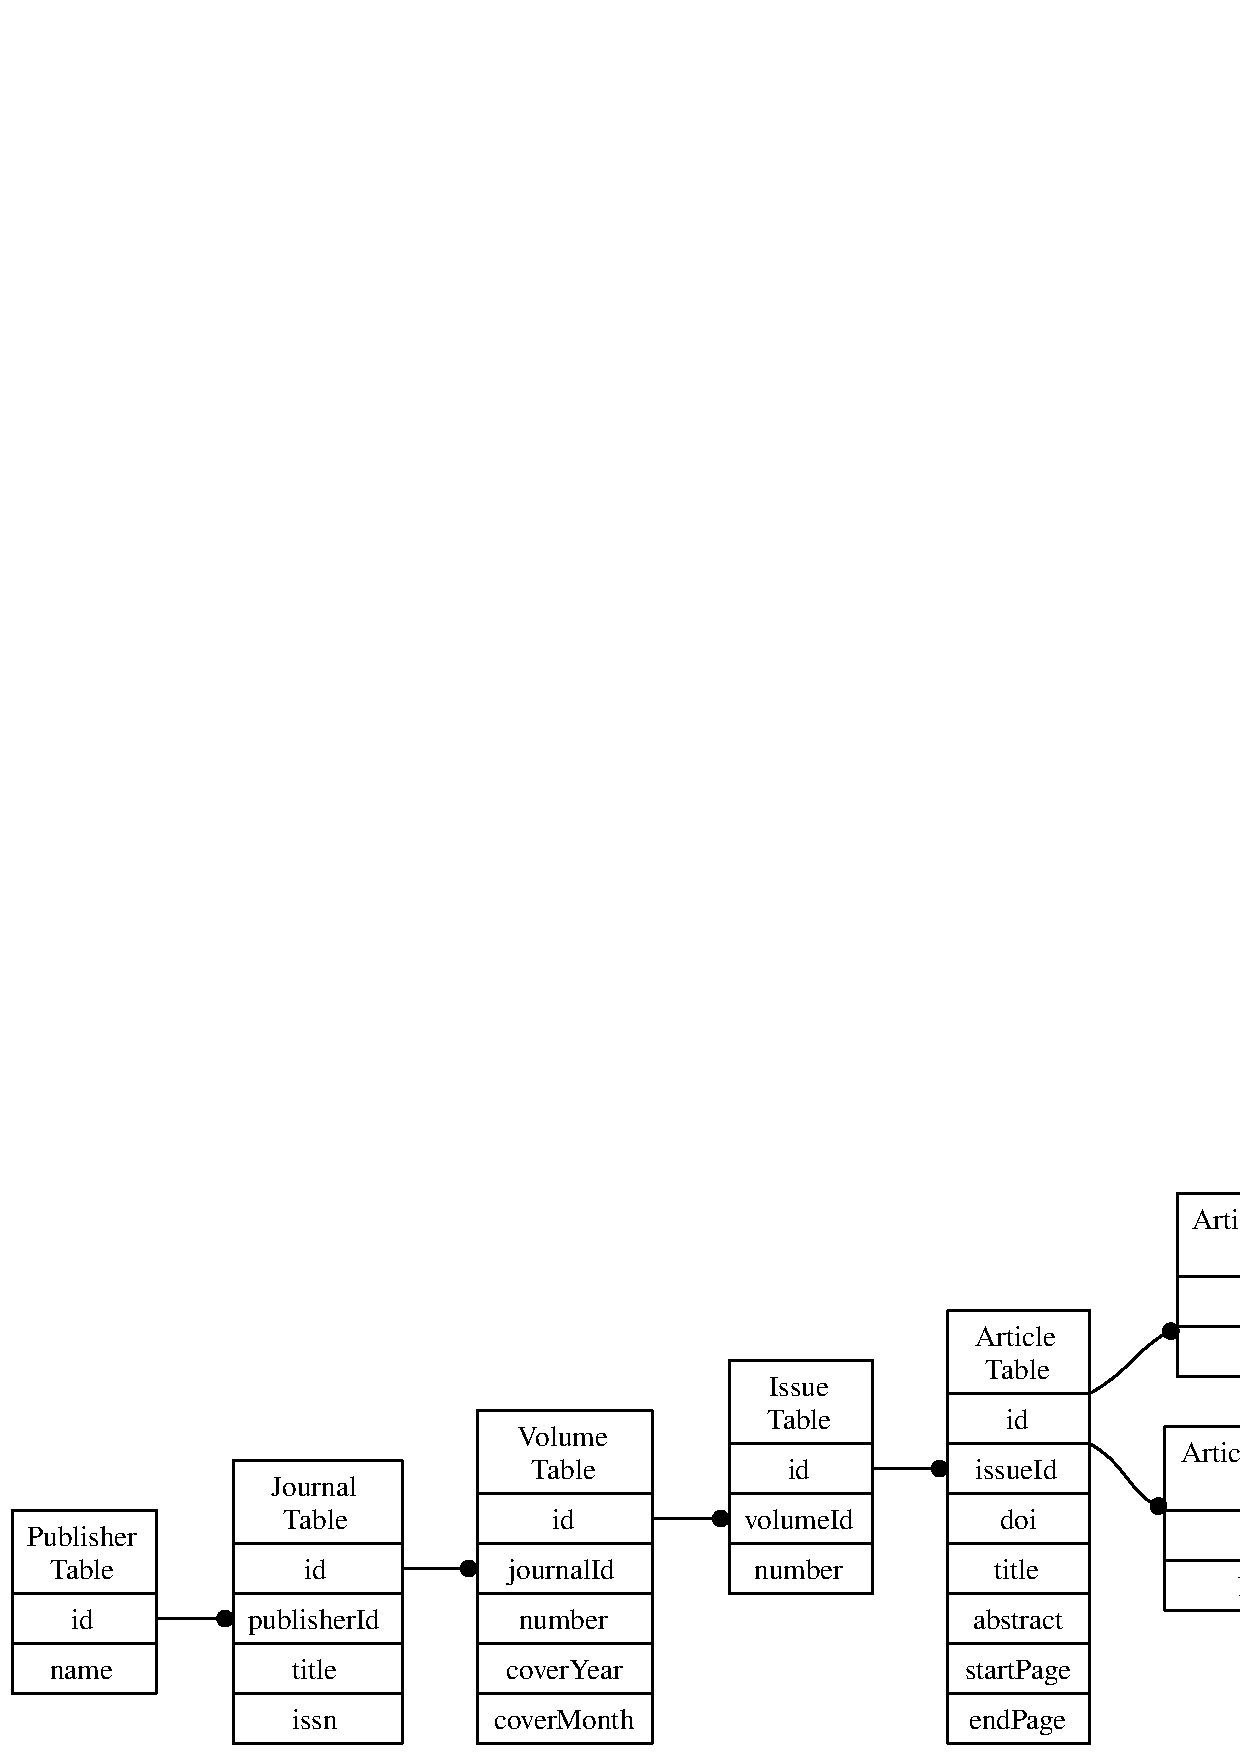
\includegraphics[width=19cm]{dot/tables.png}
%    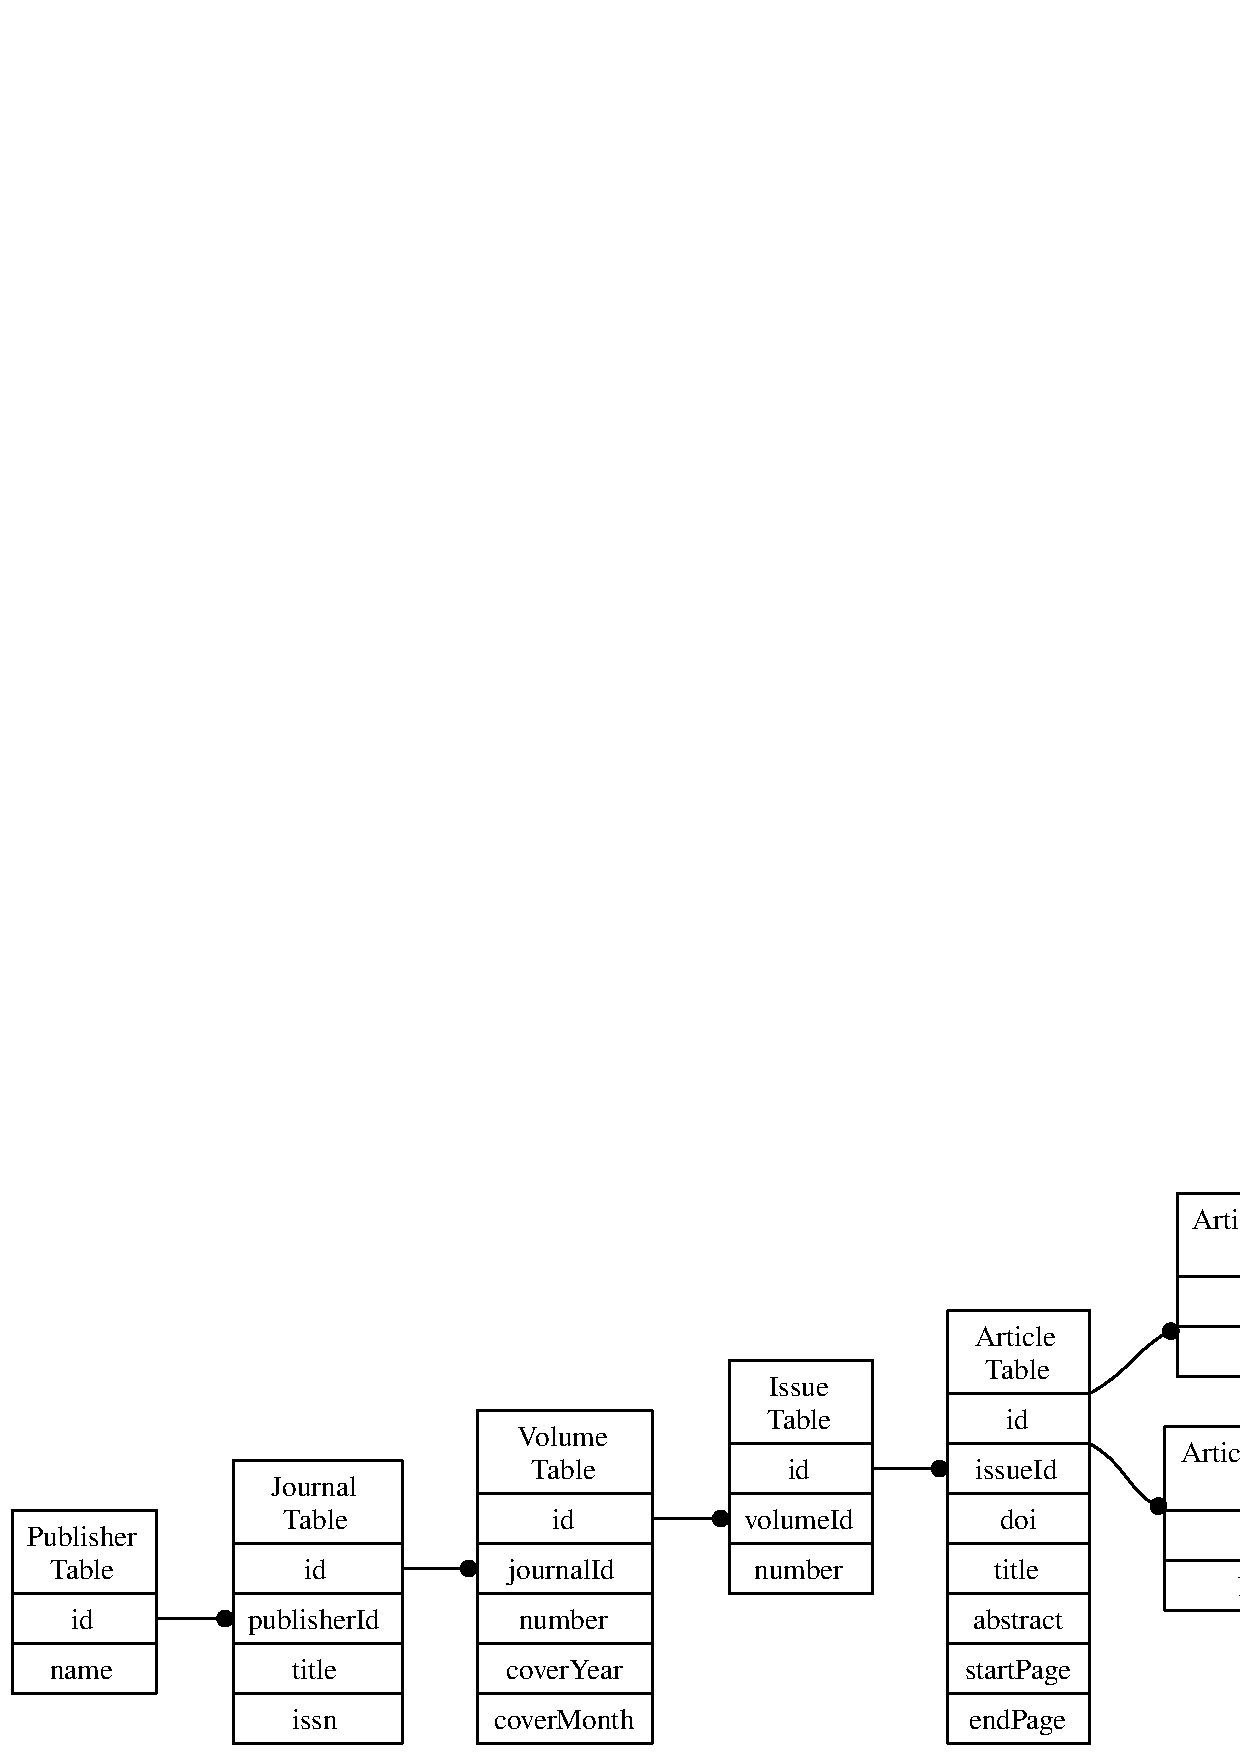
\includegraphics[width=\textwidth]{dot/tables.png}
 %   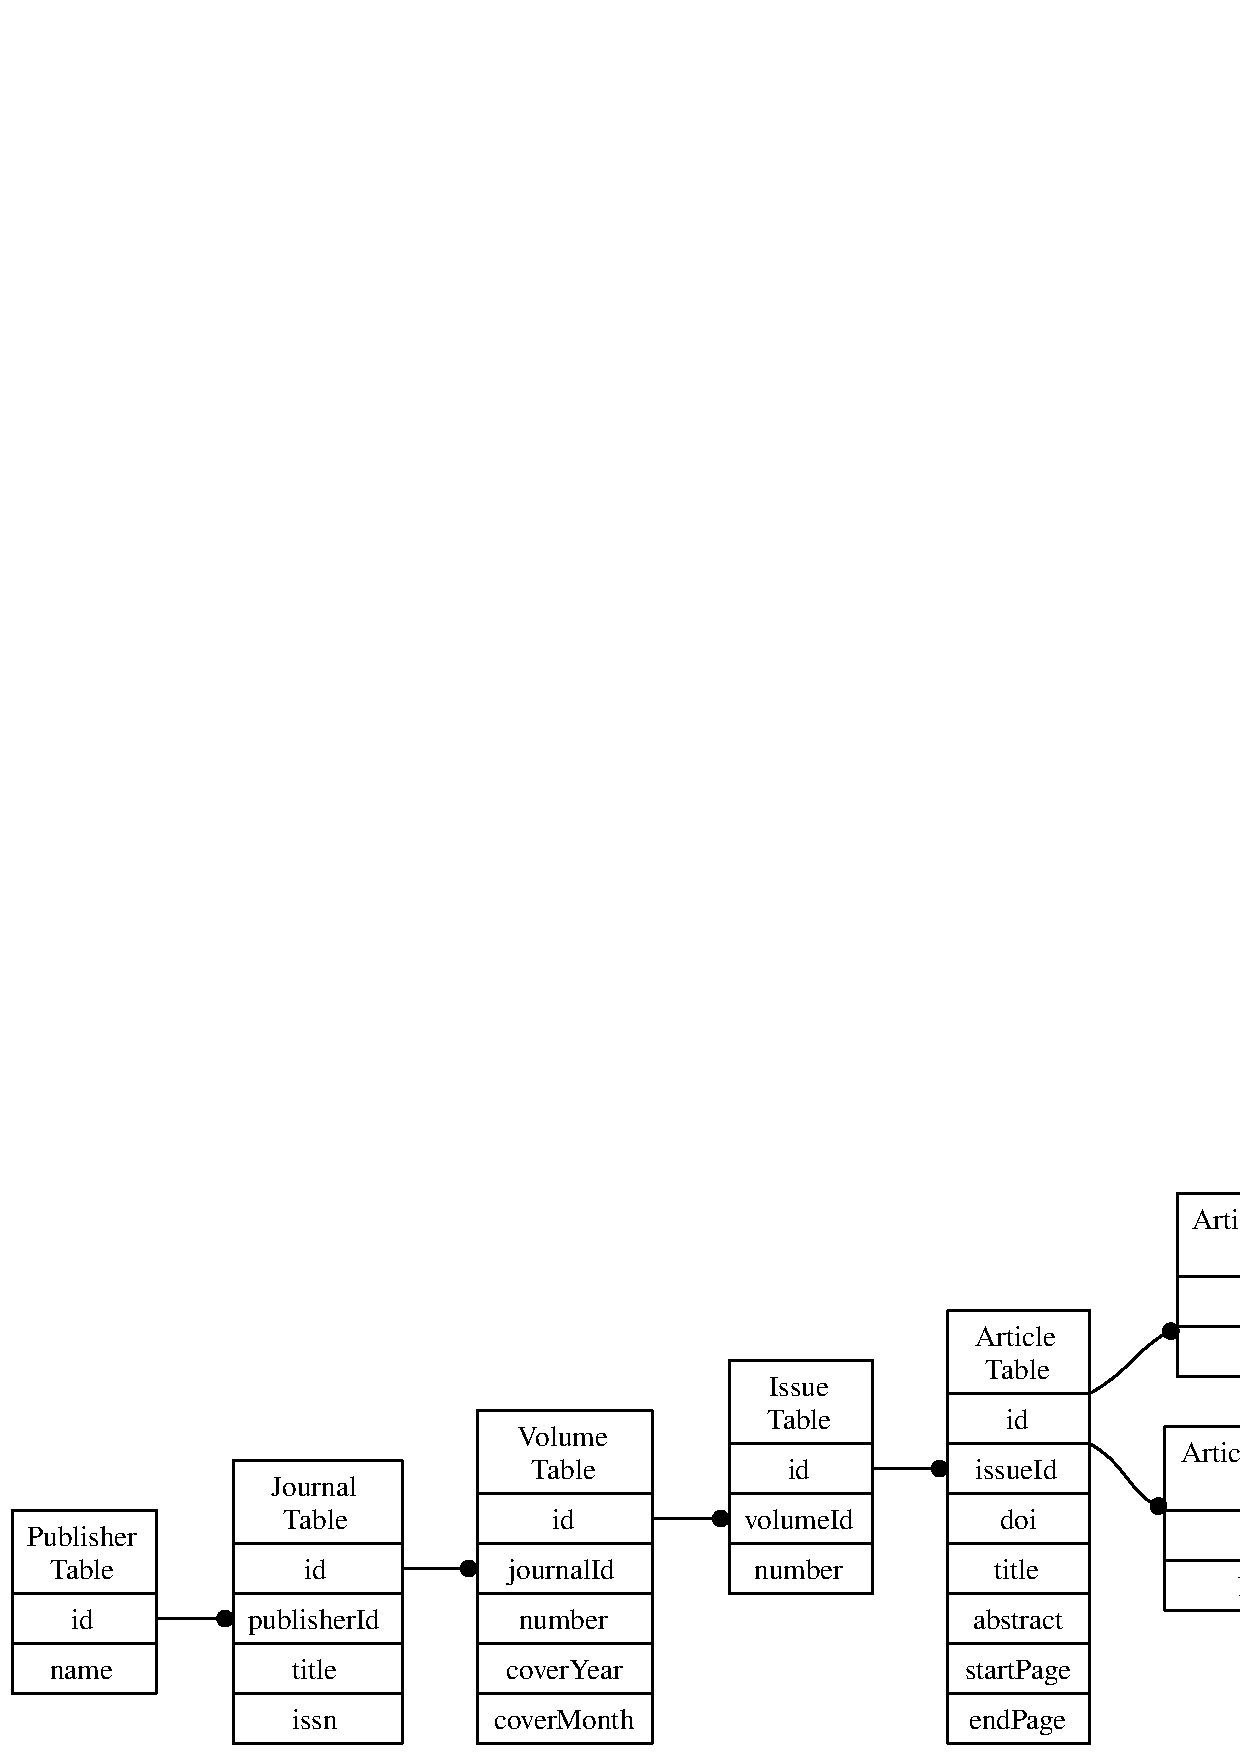
\includegraphics[width=\textheight]{dot/tables.png}
%    \makebox[\textwidth]{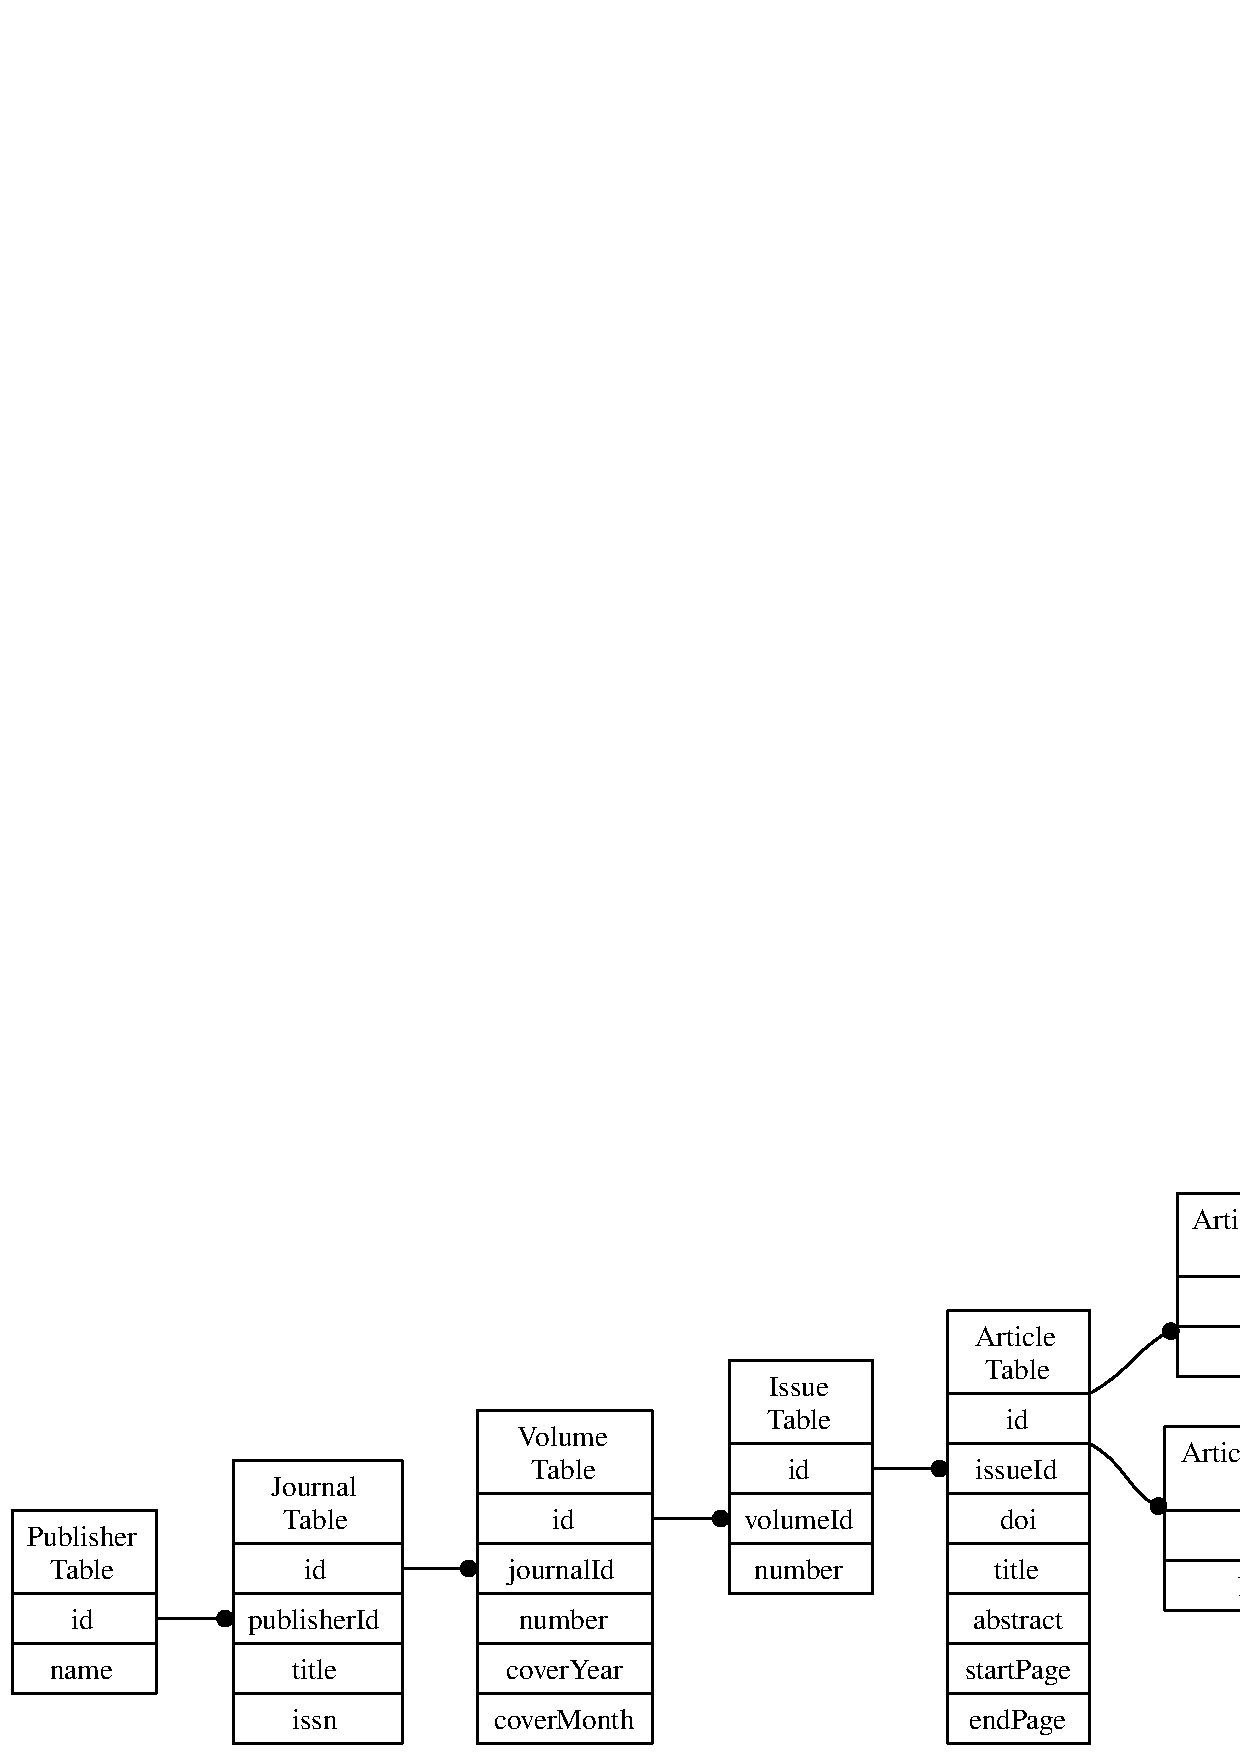
\includegraphics[width=1.15\textwidth]{dot/tables.png}}
  \end{center}
  \caption{Table relationships in Journal Article database}
  \label{tables}
\end{figure}
\end{landscape}



%%%%%%%%%%%%%%%%%%%%%%%%%%%%%%%%%%%%%%%%%%%%%%%%%%%%%%%%%%%%%%%%%%%%


\subsection[Example 2]{Example 2: Multiple tables with joins}
\label{example2}
In this example we use a fairly complex real world example to show some of the
use cases that LuSql can handle.
The database we are going to use is one that would be used to represent
journal articles.
We will use this database for the rest of the examples.
Note that the {\tt Article} table used in these examples is different from the
one used in Example 1.

Figure \ref{tables} shows the example journal article database, with tables
representing publishers, journals, volumes, issues, articles, references
(citations) authors, and keywords. 
The database represents a hierarchy (publisher {\tt hasOneOrMore} journals
{\tt hasOneOrMore} volumes {\tt hasOneOrMore} issues {\tt hasOneOrMore}
 articles) through a series of 1:N relations,
with M:N relations between articles, and authors and keywords respectively,
and a 1:N relationship for articles and references.

For this example, we are interested in the publisher, journal, volume, issue,
article information (publisher name, journal title, journal ISSN, journal
volume, journal volume year, issue number, article id, article title, article
abstract, article start page, article end page).
In order to collect it, the SQL we will use does a series of joins across
these table.

{\small
\begin{lstlisting}[backgroundcolor=\color{grey},language=Bash]
java -jar lusql.jar -q "select  Publisher.name as pub, Journal.title as jo,\
Article.rawUrl as text, Journal.issn, Volume.number as vol,\
Volume.coverYear as year, Issue.number as iss, Article.id as id,\
Article.title as ti, Article.abstract as ab, Article.startPage as startPage,\
Article.endPage as endPage\
from Publisher, Journal, Volume, Issue, Article \
where Publisher.id = Journal.publisherId and Journal.id = Volume.journalId \
and Volume.id = Issue.volumeId and Issue.id = Article.issueId" \
-c "jdbc:mysql://dbhost/db?user=ID&password=PASS" \
-n  50000 -l tutorial-2
\end{lstlisting}
}
Appendix \ref{example2-output} shows the output from this command.
You will notice one difference from the output of Example 1: 
{\small
\begin{lstlisting}[backgroundcolor=\color{grey},language=Bash]
.......... 10000 docs    5s                                                                                   
.......... 20000 docs    3s                                                                                   
.......... 30000 docs    4s                                                                                   
.......... 40000 docs    5s                                                                                   
.......... 50000 docs    5s                                                                                   
\end{lstlisting}
}
With the verbose output, LuSql provides a progress indicator and prints out a
period for each 1000 documents it indexes.
It then prints a total and a time to index, for each 10,000 documents indexed.


\subsubsection{Example 2 examined in Luke}
Again, we examine the index with Luke:
\begin{mlist}
\item Figure \ref{luke_2_1} shows the {\tt Overview} panel, showing the 50,000 {\tt
    Document}s have been added.
\item Figure \ref{luke_2_2} shows the {\tt Document} panel, showing the fields
  derived from the SQL join.
\item Figure \ref{luke_2_3} shows a search and two resulting {\tt Documents}. 
  The search reveals an underlying data problem with the original DBMS, as
  these two {\tt Document}s are the same article, with the only difference
  with one having an issue number of {\tt 1} with the other having an issue
  number of {\tt none}.
  Otherwise this index is behaving as expected.
\end{mlist}

%\begin{landscape}
  \begin{figure}
  \begin{center}
 % \includegraphics[height=\textwidth]{images/luke_2_1.png}
 \includegraphics[width=\textwidth]{images/luke_2_1.png}
      \end{center}
  \caption{Example 2 in {\tt Luke}: Overview panel}
\label{luke_2_1}
\end{figure}
%\end{landscape}
%\begin{landscape}
  \begin{figure}
  \begin{center}
%  \includegraphics[height=\textwidth]{images/luke_2_2.png}
  \includegraphics[width=\textwidth]{images/luke_2_2.png}
      \end{center}
  \caption{Example 2 in {\tt Luke}: Documents panel}
\label{luke_2_2}
\end{figure}
%\end{landscape}
%\begin{landscape}
\begin{figure}
  \begin{center}
%    \includegraphics[height=\textwidth]{images/luke_2_3.png}
    \includegraphics[width=\textwidth]{images/luke_2_3.png}
  \end{center}
  \caption{Example 2 in {\tt Luke}: Search panel}
  \label{luke_2_3}
\end{figure}
%\end{landscape}


\subsection[Example 3]{Example 3: Multiple tables with joins and additional
  subqueries} 
\label{example3}
We continue using the journal article database.
If we were really wanting to create a useful Lucene index for journal
articles, one of the things that would certainly be needed would be the
ability to search articles by authors and/or keywords, or to navigate by
references. 
However, the Lucene index created with Example 2 does not offer this, and
indeed the functionality presented up to now of LuSql does not allow
us to make this sort of index.

LuSql, however, does offer additional functionality to do this sort of thing.
For each {\tt Document}\footnote{Internally, LuSql does not use Lucene {\tt
    Document}s until just before sending the information to be indexed. 
  Instead, LuSql uses its own abstraction for a document, {\tt Doc}, which
  described in Section \ref{doc}.} 
created from the original SQL query, one or more
additional queries can be formulated and run to obtain additional information
from the DBMS and add this to the {\tt Document}. 
These additional queries are constructed by defining a field from the original
query results which is used as a linking key in the additional queries. 

In our example, we want the field {\tt id} from the {\tt Article} table to be used
in SQL queries to get the author, keyword and reference information from their
respective tables.
The relationship between {\tt Article} and both {\tt Author} and {\tt
  Keyword} is many--to--many, with each table having a join table to handle
this relationship ({\tt ArticleAuthorJoin} and {\tt ArticleKeywordJoin},
respectively). 
The relationship between {\tt Article} and {\tt Reference} is a one--to--many.

The queries to select the appropriate authors, keyword and references for a
particular article, say
{\tt Article.id=3453}, would therefor be:
\begin{lstlisting}[backgroundcolor=\color{grey},language=SQL]
select Keyword.string as keyword 
 from ArticleKeywordJoin, Keyword
 where ArticleKeywordJoin.articleId=3453 and
 and ArticleKeywordJoin.keywordId = Keyword.id;

select concat(lastName,', ', firstName) as fullAuthor 
 from ArticleAuthorJoin, Author
 where ArticleAuthorJoin.articleId = 3453 
 and ArticleAuthorJoin.authorId = Author.id;

select referencedArticleId as citedId 
 from Reference 
 where Reference.referencingArticleId = 3453;
\end{lstlisting}


LuSql supports this sort of subquery through an additional command line
parameter {\tt-Q}.
This parameter takes a field from the main query whose value is used as a key
in the subqueries.
In the above example, these would be {\tt Article.id} and 3453, respectively.

When constructing the SQL query, the metavariable {\tt @} is used in the
place where the key value literal would be used.
When LuSql is run, the {\tt @} is replaced with the value of the
field name ({\tt fieldName}) from each {\tt Document} object and any fields
returned (via records) are added to the {\tt Document}. 



Here is how the {\tt -Q} parameters would look like in our example (just add
the below to the LuSql command shown in Example 2, Section \ref{example2}):

\begin{lstlisting}[backgroundcolor=\color{grey},language=SQL]
 -Q "id|select Keyword.string as keyword from ArticleKeywordJoin, Keyword\
  where ArticleKeywordJoin.keywordId=@\ 
  and ArticleKeywordJoin.articleId = Keyword.id"\
 -Q "id|select concat(lastName,', ', firstName) as fullAuthor\
  from ArticleAuthorJoin, Author where ArticleAuthorJoin.articleId = @\
  and ArticleAuthorJoin.authorId = Author.id"\
 -Q "id|select referencedArticleId as citedId\
  from Reference where Reference.referencingArticleId = @"
\end{lstlisting}

Note that the {\tt concat(lastName,', ', firstName)} construct used in the
author query is a MySQL specific function\footnote{
\url{http://dev.mysql.com/doc/refman/5.0/en/string-functions.html}{function\_concat}}.

The {\tt -Q} parameter has the following three variants:
\begin{mlist}
\item {\tt -Q "fieldName|SQL"} --- as per the above example.
\item {\tt -Q "fieldName|NNN|SQL"}
\item {\tt -Q "fieldName|NNN NNN...NNN|SQL"}
\end{mlist}

In the first variant, the {\tt NNN} is left out altogether, and the {\tt NNN} for all
fields for this query are taken from the default value or the value set by the
global {\t -I} (see Section \ref{nnn}).
In the second form, the  {\tt NNN} is the Lucene {\tt Field} index/store/term vector
attributes for all fields returned by the subquery.
In the third form, there is a corresponding {\tt NNN} for each of the fields.



Appendix \ref{example3-output} shows the output for Example 3.

\subsubsection{Example 3 examined in Luke}
Here we will briefly look at the index using Luke.
In Figure \ref{luke_3_1} we can see a document showing the additional fields
added by the {\tt -Q} subqueries ({\tt author, citeId, keywords}).
  \begin{figure}
  \begin{center}
 \includegraphics[width=\textwidth]{images/luke_3_1.png}
      \end{center}
  \caption{Example 3 in {\tt Luke}: Documents panel}
\label{luke_3_1}
\end{figure}

%% {\tt 
%% -Q  "id:select Keyword.string as keyword 
%%  $\backslash$\newline
%% from ArticleKeywordJoin, Keyword
%%  $\backslash$\newline
%%  where ArticleKeywordJoin.articleId=@
%%  $\backslash$\newline
%% ArticleKeywordJoin.authorId = Keyword.id"
%% }

%\end{landscape}



\subsection[Example 4]{Example 4: Multiple tables with joins, additional
  queries and filter}
\label{example4}
We continue using the journal article database.
In our journal article database, the article {\em metadata} is kept in the
database, but the full-text of the article is kept in the filesystem in a text
file (extracted from the PDF or supplied by the publisher).
The convention for the path of this file is:\\
{\tt issn/volumeNumber/issueNumber/start-page/arbitraryFileName.txt.gz}.
The field {\tt Article.rawUrl} contains this path, less the {\tt .gz} suffix,
as the files are compressed to save disk space.
So, to create an index that would allow search of the full-text as well as the
metadata, we need to get the full-text content from the filesystem into the 
Lucene index.

LuSql provides a plugin mechanism that allows for arbitrary manipulation of
{\tt Doc}s after they are populated from the database, after any 
{\tt  -Q} additional queries, and before the {\tt Doc} is indexed.
Section \ref{filter} describes how to implement filters ({\tt
  DocFilters}), and Appendix \ref{filterSource} shows the implementation
that we use here to construct the file path, open and un--gzip the file,
read the text from the file into a {\tt String} then add this string 
to the {\tt Doc}, with {\tt Field.Index.TOKENIZED,
Field.Store.YES,\footnote{In a real example, the full-text would likely, not be
  stored, especially in very large collection indexes. In this case, the
  full-text is stored so it can be perused using Luke} Field.TermVector.YES}). 


As this example uses both a filter and subqueries, this may be a good time to
describe the order in which these various things occur in LuSql.
Below is simple pseudocode describing the process:

\begin{lstlisting}[backgroundcolor=\color{grey}]
   foreach resultSet
   {
       make Doc From ResultSet;
       run SubQueries;
       run Filter;
       convert Doc to Lucene Document;
       add Document To Lucene Index;
   }
   run Filter.onDone;
   close Lucene and JDBC Connection;
   optimize Lucene index;
\end{lstlisting}

Appendix \ref{filterSource} shows a filter which implements what we described
above to index the filesystem full-text.
The {\tt -f} command line parameter indicates the filter class to use. 
Append the following text to the command line from Example 3,
Section \ref{example3}) to use the filter we have implemented:
{\small
\begin{lstlisting}[backgroundcolor=\color{grey}]
 -f ca.nrc.cisti.lusql.example.FileFullTextFilter   
\end{lstlisting}
}

Appendix \ref{example4-output} shows the output from this invocation of LuSql.


\subsubsection{Example 4 examined in Luke}
Here we will briefly look at the index using Luke.
In Figure \ref{luke_4_1} we can see a document showing the additional field
added by the filter ({\tt fulltext}.
  \begin{figure}
  \begin{center}
 \includegraphics[width=\textwidth]{images/luke_4_1.png}
      \end{center}
  \caption{Example 4 in {\tt Luke}: Documents panel}
\label{luke_4_1}
\end{figure}


\section{Filter plugin}
\label{filter}
LuSql offers a plugin architecture which allows the user to define a
class which has access to the {\tt Doc} after it is created but
before it is converted into a Lucene {\tt Document} and this is indexed. 
This allows arbitrary modification of the {\tt Doc} object.


\subsection{Interface {\tt DocFilter}}
A class implementing {\tt DocFilter} only needs to implement the
two methods shown below.
\begin{lstlisting}[backgroundcolor=\color{grey},language=Java]
public interface DocFilter 
{
    public Doc filter(Doc doc); 
    public void onDone();
    public void setProperties(Properties filterProperties);
}
\end{lstlisting}

\subsubsection{Class {\tt Doc}}
\label{doc}
{\tt Doc} is an interface that is LuSql's internal abstract
representation of a document, that exposes a number of methods to allow manipulation:
\begin{lstlisting}[backgroundcolor=\color{grey},language=Java]
public interface Doc 
{
   public void addField(final String name, String value, LuceneFieldParameters lfp);
   public LuceneFieldParameters getFieldParameters(String field);
   public void addFieldParameters(String[] fieldNames, LuceneFieldParameters[] paras);
   public void addField(final String name, String value);
   public void addFieldParameter(String field, LuceneFieldParameters paras);
   public void populate(ResultSet rs, String[] fieldNames) throws SQLException;
   public boolean containsField(String key);
   public void removeField(String name);
   public Iterator<String> getFieldNames();
   public List<String> getFieldValues(String key);
   public void clear();
}
\end{lstlisting}

\subsubsection{Class {\tt LuceneFieldParameters}}
The LuSql class {\tt LuceneFieldParameters} used above is a container class for the
three Lucene {\tt Field} parameters and has the following constructor:
\begin{lstlisting}[backgroundcolor=\color{grey},language=Java]
    public LuceneFieldParameters(Field.Index newIndex,
				 Field.Store newStore,
				 Field.TermVector newTermVector) 
\end{lstlisting}




\subsection{Interface {\tt DBDocFilter}}
Sometimes the class implementing {\tt DocFilter} needs to access
the SQL database being used.
{\tt DBDocFilter} is an interface that extends  {\tt
  DocFilter} and offers access to the {\tt DataSource} object so
it can be used by the filter.
The {\tt DBDocFilterImp} class implements this interface, so
developers can just extend this class to get this functionality.

\begin{lstlisting}[backgroundcolor=\color{grey},language=Java]
public interface DBDocFilter 
    extends DocFilter 
{
    public void setDataSource(DataSource ds);
    public DataSource getDataSource();
}
\end{lstlisting}

See Appendix \ref{filterSource} for an example implementation.














\section{Performance}

\subsection{Tuning}
\subsubsection{Java VM options}
\begin{mlist}
\item {\tt -XX:+AggressiveOpts} was found to increase thoughput on this configuration.
\end{mlist}

\subsubsection{Lucene indexing}
Using large RAM buffer makes indexing faster. 
However, with very large RAM buffer size, the delay in flushing the buffer can
be longer than the JDBC connection is comfortable with, and can cause a
timeout. 
This can be solved by setting rather small RAM buffer sizes, like the Lucene
default value of 16MB.

\subsubsection{SQL Database and queries}
\begin{mlist}
\item Make sure fields that are used in {\tt WHERE} clauses are appropriately indexed.
\end{mlist}

\paragraph{MySQL}
\begin{mlist}

\item Add {\tt cacheResultSetMetadata=true}\footnote{\url{http://dev.mysql.com/doc/refman/5.0/en/connector-j-reference-configuration-properties.html}} 
  to the connection String for MySql. 
\end{mlist}


\subsection{Indexing Performance}
Here is the indexing performance for examples 2--4 of the tutorial in
Section \ref{tutorial}, indexing all of the records (6,409,484) from each
query.  

\subsubsection{Example 2}
Total indexing time: {\bf 5675s (1h 34m 35s)} \\
Optimizing time: {\bf 2725s (m s)} \\
Index size: {\bf 21GB} \\

\noindent LuSql command:
\begin{lstlisting}[backgroundcolor=\color{grey},language=Bash]
java -XX:+AggressiveOpts -Xms1000m -Xmx1000m\
 -jar lusql.jar  -q "select Article.id as id,\
 Article.title as ti, Article.abstract as ab,\
 Publisher.name as pub, Journal.title as jo,\
 Journal.issn,Volume.number as vol,\
 Volume.coverYear as year, Issue.number as iss,\
 Article.doi as doi,Article.title as title,\
 Article.abstract as abstract, Article.startPage as startPage,\
 Article.endPage as endPage from Publisher, Journal,\
 Volume, Issue, Article where Publisher.id=Journal.publisherId\
 and Journal.id = Volume.journalId and Volume.id\
 =Issue.volumeId and Issue.id = Article.issueId " -c\
 "jdbc:mysql://dbhost/db?user=USER&password=PASS"\
 -v -l example2-large
\end{lstlisting}


\subsubsection{Example 3}
Total indexing time: {\bf 14750s (4h 4m 50s)} \\
Optimizing time: {\bf 2260s (37m 40s)} \\
Index size: {\bf 22GB} \\

\noindent LuSql command:  \\
Like Example 2, with  {\tt -l example3-large} and appending:
\begin{lstlisting}[backgroundcolor=\color{grey},language=Bash]
-Q "id|select string as keyword from Keyword,\
 ArticleKeywordJoin where ArticleKeywordJoin.articleId = @\
 and ArticleKeywordJoin.keywordId = Keyword.id"\
-Q "id|select lastName, firstName from Author,\
 ArticleAuthorJoin where ArticleAuthorJoin.articleId = @\
 and ArticleAuthorJoin.authorId = Author.id"\
-Q "id|select referencedArticleId as citedId\
 from Reference where Reference.referencingArticleId = @"
\end{lstlisting}

\subsubsection{Example 4}
{\bf NB}: There was not sufficient disk space on the indexing machine to
index. 
Instead, the indexing was done on the database machine.
As both the indexing and database were running in the same machine, it is
almost certain that the indexing time would be significantly less than for the
previous examples, so making comparisons between these results and results
from Examples 2 and 3 would not be appropriate. \\

\noindent Total indexing time: {\bf 49593 s (13h 46m 33s)} \\
Optimizing time: {\bf 9623s (2h 40m 23s)} \\
Index size: {\bf 86GB GB}

\noindent LuSql command:  \\
\noindent Like Example 3 with {\tt -l example4-large}, and appending
\begin{lstlisting}[backgroundcolor=\color{grey},language=Bash]
 -f ca.nrc.cisti.lusql.example.FileFullTextFilter
\end{lstlisting}










\section{Acknowledgements}

I would like to thank the following people who helped in various ways:
 Andre Vellino, the first LuSql customer, and supportive bug discoverer;
 Greg Kresko, zealous proof--reader and CISTI Research sysadmin support;
 those developing Lucene directly (Doug Cutting, Erick Hatcher et al.);
 Andrzej Bialecki for creating Luke;
 the participants of the Lucene user list\footnote{\url{http://mail-archives.apache.org/mod_mbox/lucene-java-user}}. 


\noindent I would also like to acknowledge the support of my employer, NRC CISTI.


\newpage
\appendix
\section{LuSql license, copyright and authorship}

\subsection{Documentation License}
This document is licensed under the
Creative Commons Attribution-Share Alike 2.5 Canada 
License\footnote{\url{http://creativecommons.org/licenses/by-sa/2.5/ca/}}.


\subsection{Software License}
The LuSql software is licensed under the 
Apache License v2\footnote{\url{http://www.apache.org/licenses/LICENSE-2.0.txt}}.

\begin{center}
  \includegraphics[width=2.5cm]{images/apache-feather-small.png}
\end{center}

\subsection{Copyright}
The LuSql software is \copyright \ 2008  National Research Council Canada


\subsection{Author}
The author of the LuSql software is
\href{http://lab.cisti-icist.nrc-cnrc.gc.ca/cistilabswiki/index.php/Glen_Newton}{Glen
  Newton}\footnote{\url{http://lab.cisti-icist.nrc-cnrc.gc.ca/cistilabswiki/index.php/Glen_Newton}}, Researcher, CISTI, NRC.

\noindent {\tt \href{mailto:glen.newton@nrc-cnrc.gc.ca}{glen.newton@nrc-cnrc.gc.ca}}.




\newpage
\section{TODO}
\label{todo}
Here are a number of features planned for future versions.
This list is not exhaustive, and will be altered by user feedback.

\subsection{{\tt Properties} for command line arguments}
The LuSql command line can get quite complicated for any non-trivial usage.
With the additional functionality described in this list, it is likely to
become more complex. 
Being able to optionally put some or all of the configuration
described in the command line parameters in a {\tt Properties} file would be
useful. 

\subsection{Test on other DBMS}
Only MySql has been tested for v0.9.
Other databases should be tested, such as IBM's 
DB2, PostgreSql, Oracle, Derby, H2, etc.
Prioritize?

\subsection{Updating}
\begin{mlist}
\item Ability to indicate a field in previously created LuSql Lucene index as a
primary key into the SQL {\tt ResultSet}, and use this key to do updates (i.e. query
Lucene for the {\tt ResultSet} key field value; if not in Lucene add, otherwise move
to the next {\tt ResultSet}).

\item An automatically added timestamp field to be used for updates would also
  be useful. 
  I guess this can be done now with {\tt -g}.
\end{mlist}




\subsection{Logging, JUnit}
Need to add:
\begin{mlist}
\item Logging
\item JUnit tests
\end{mlist}

\subsection{Refactor {\tt LuSql.java}}
{\tt LuSql.java} is a blob and needs to be refactored into several more OO,
more testable and more independent classes.
\begin{mlist}
\item Central way to set default JDBC Connection, ResultSet, Statement values
\item Get rid of {\tt -j} cruft (deprecated).
\item Others...
\end{mlist}

\subsection{Robust Connection Failure Handling}
In v0.9, if the JDBC connection fails, LuSql re-issues the query and loops
over the {\tt ResultSet} until it gets to qwhere it left off.
It then contunues indexing.
However, this functionality was a late addition, and it is rather fragile.

Need to improve this code.
Refactoring of {\tt LuSql} class will help.

\subsection{Per field weighting}
Right now, all fields get the default weighting. 
Need the ability to set the field weighting.
Perhaps something like
\begin{lstlisting}[backgroundcolor=\color{grey}]
-w "id 0.75"  -w "author 0.90"
\end{lstlisting}



\subsection{Extend Subquery Functionality}
\begin{mlist}

\item Right now, subqueries are limited to the same database as the core query.
There are use cases where the subquery needs to query another database, even
on a different DBMS on a different machine (different connect URL, different
driver).
As this gets rather complicated, perhaps too complicated to add to the command
line ar, this user access to this yet unimplemented functionality
configuration will likely be pushed to the {\tt Properties}, above.

Implications: access to these additional {\tt DataSource} might be needed in
{\tt DBDocFilter}. Perhaps an abstract subclass with abstract methods
\begin{lstlisting}[backgroundcolor=\color{grey},language=Java]
public class MultipleDBDocFilter
    public void setDataSource(String key, DataSource ds);
    public DataSource getDataSource(String key);
\end{lstlisting}


\item Right now, subqueries are run before the {\tt DocumentFilter}. 
Need to be able to have run after using a command line argument toggle.

\end{mlist}

\subsection{Multiple Analyzers}
\hypertarget{analyzer}
Right now (v0.9) a single {\tt Analyzer} is applied to all fields.
Need to allow for more than a single {\tt Analyzer}, i.e. the ability to map 
  database record fields to different {\tt Analyzers}.
Again, probably so complex need to do using {\tt Properties} file.
Possible command line parameters:
\begin{lstlisting}[backgroundcolor=\color{grey},language=Java]
  -b "id org.apache.lucene.analysis.standard.SimpleAnalyzer"\  
  -b "author org.apache.lucene.analysis.standard.SimpleAnalyzer" 
\end{lstlisting}

%\subsection{Use SOLR configuration}


\subsection{Abstract data source}
An abstract data source pluggable should be implemented, like SOLR's
{\tt DataSource}\footnote{\url{http://lucene.apache.org/solr/api/org/apache/solr/handler/dataimport/DataSource.html}}
and {\tt
  DataImportHandler}\footnote{\url{http://wiki.apache.org/solr/DataImportHandler}}.

\subsubsection{SPARQL}
In addition to SQL and JDBC, extend to allow SPARQL\footnote{\url{http://en.wikipedia.org/wiki/SPARQL}}
queries of a SPARQL
end--point\footnote{\url{http://semanticweb.org/wiki/SPARQL_endpoint}} 
and index the results.
This could be done as a plugin.



\subsection{Abstract indexing: data sink}
The complement to the previous entry: have an abstract plug-in model for
indexing, so other indexing technologies in addition to Lucene can be dropped
in, such as Minion{\footnote{\url{https://minion.dev.java.net}},
Xapian\footnote{\url{http://www.xapian.org}} (through Java bindings),
Terrier\footnote{\url{http://ir.dcs.gla.ac.uk/terrier}},
MG4J\footnote{\url{http://mg4j.dsi.unimi.it}} (Managing Gigabytes for Java),
Lemur\footnote{\url{http://www.lemurproject.org}} (through Java bindings),
etc. 


\subsection{Alternatives for storage}
For some use cases, using Lucene to store content may not be the best
solution.
For example, storing large volumes of content in very large Lucene indexes
that need to be highly performant will see reduced performance due to this
storage.
Instead, putting the content in a simpler, faster content system such as 
Berkeley
DB\footnote{\url{http://www.oracle.com/technology/products/berkeley-db/index.html}},   
Tokyo Cabinet\footnote{\url{http://tokyocabinet.sourceforge.net/index.html}},
QDBM\footnote{\url{http://qdbm.sourceforge.net}}, or to an embedded DBMS, such
as H2\footnote{\url{http://www.h2database.com}}, 
Derby\footnote{\url{http://db.apache.org/derby}},
or HSQLDB\footnote{\url{http://hsqldb.org}}, 
or even back into a client-server DBMS might be a better technical solution. 

All fields marked {\tt Field.Store.YES} using the {\tt NNN} syntax, do not
store them in Lucene but store them using some other persistance technology,
with an agreed--upon key to get the stored document. Have a plugin model for
storing documents, while still indexing them with Lucene. 

What about fields marked {\tt Field.Store.COMPRESS}? gzip first then store?



\subsection{Multiple Parallel Indexes}
Option to have multiple parallel indexes that are merged into a single index
at the end of the indexing (needs approximately double the disk space).

\subsection{Update to Lucene 2.4}
\subsubsection{New and deprecated {\tt Field.Index}}
Lucene 2.4 has added a new designation and changed the names of {\tt
  Field.Index}: \\
\noindent{\bf New\footnote{\url{http://lucene.apache.org/java/2_4_0/api/org/apache/lucene/document/Field.Index.html}}}\\
{\tt Field.Index.ANALYZED\_NO\_NORMS} \\
\noindent{\bf Deprecated:} \\
{\tt Field.Index.TOKENIZED} renamed {\tt Field.Index.ANALYZED} \\
{\tt Field.Index.UN\_TOKENIZED} renamed  {\tt Field.Index.NOT\_ANALYZED} \\
{\tt Field.Index.NO\_NORM} renamed {\tt
Field.Index.NOT\_ANALYZED\_NO\_NORMS}


\subsection{Apache Commons DBCP}
Need parameter to control the number of connections, initial size, wait time,
etc in the pool.
Right now, it uses the default
values\footnote{\url{http://commons.apache.org/dbcp/configuration.html}}. 




\subsection{Roadmap}
\subsubsection{V1.0}
Bug fixes.

\subsubsection{V1.01}
Code clean-up; refactor; bug fixes.
\subsubsection{V1.02}
Update to Lucene 2.4.x.

\subsubsection{V1.03}
{\tt Properties}

\subsubsection{V1.04}
Multiple analyzers.


\subsection{Changes}
\subsubsection{v0.9 2008 11 10}
Initial Release.

\newpage
\section{Indexing Parameters for arguments {\tt -i} and {\tt -I}}
\label{parameters}
These also apply to some other command line arguments, like {\tt -Q}.
The default value is {\bfseries \tt 211} or {\tt Field.Index.TOKENIZED, Field.Store.YES, Field.TermVector.YES}.

\subsection{\tt Field.Index}

\begin{table}[h]
\begin{center}
\label{tableIndex}
\begin{tabular}{|c|l|c|}
\hline
\bfseries Option value & {\bfseries \tt Field.Store} value&Default?\bfseries \\ \hline \hline
        0&\tt NO & \\ \hline
        1&\tt NO\_NORMS& \\\hline
        2&\tt TOKENIZED& $\surd$\\\hline
        3&\tt UN\_TOKENIZED& \\\hline
\end{tabular}
\end{center}
\end{table}



\subsection{\tt Field.Store}
\begin{table}[h]
\begin{center}
\label{tableStore}
\begin{tabular}{|c|l|c|}
\hline
\bfseries Option value & {\bfseries \tt Field.Store} value&Default?\bfseries \\ \hline \hline
        0&\tt NO& \\ \hline
        1&\tt YES&$\surd$ \\ \hline
        2&\tt COMPRESS&\\ \hline
\end{tabular}
\end{center}
\end{table}






\subsection{\tt Field.TermVector}
\begin{table}[h]
\begin{center}
\label{tableVector}
\begin{tabular}{|c|l|c|}
\hline
\bfseries Option value & {\bfseries \tt Field.TermVector} value&Default?\bfseries \\ \hline \hline
        0& \tt NO&  \\\hline
        1& \tt YES & $\surd$\\\hline
        2& \tt WITH\_OFFSETS & \\\hline
        3& \tt WITH\_POSITIONS & \\\hline
        4& \tt WITH\_POSITIONS\_OFFSETS & \\\hline
\end{tabular}
\end{center}
\end{table}


\newpage
\section{Hardware, software, OS used in examples}
\label{hardware}

The configuration consisted of an indexing machine and a DBMS machine.
LuSql was run from the indexing machine.
For Example 4, the full-text files were stored on the storage array described
below. 

\subsection{Hardware}
\noindent {\bf Indexing and database machines}: \\
{\bf Dell PowerEdge 1955 Blade server}\footnote{\url{http://www.dell.com/content/products/productdetails.aspx/pedge_1955?c=us&l=en&s=corp}}\\
\indent {\bf CPU}: 2 x dual-core Xeon 5050 processors with 2x2MB cache, 3.0 GHz\\
\indent {\bf Memory}: 8 GB 667MHz\\
\indent {\bf Disk:} 2 x 73GB internal 10K RPM SAS drives\\


\noindent Both machines attached to:\\
\indent Dell EMC AX150 storage arrays\\
\indent 12 x 500 GB SATA II 7.2K RPM disks\\
via:\\
\indent SilkWorm
200E\footnote{\url{http://www.brocade.com/products-solutions/products/switches/product-details/200e-switch/index.page}.
Also see the Dell site
\url{http://www.dell.com/content/products/productdetails.aspx/pvaul_ds16b4?c=us&cs=555&l=en&s=biz}}
Series 16-Port Capable 4Gb Fabric Switch.

\subsection{Software}
{\bf MySql}: v5.0.45 compiled from source.

\noindent {\bf gcc}: \\
\ gcc version 4.1.2 20061115 (prerelease) (SUSE Linux)

\noindent {\bf Java}: \\
\ java version 1.6.0\_07\\
\ Java(TM) SE Runtime Environment (build 1.6.0\_07-b06)\\
\ Java HotSpot(TM) 64-Bit Server VM (build 10.0-b23, mixed mode)

\subsection{Operating System}
Linux openSUSE 10.2 (64-bit X86-64)\\
Linux kernel: 2.6.18.8-0.10-default \#1 SMP

\newpage
\section{MySQL Tutorial Tables for Examples 2--4}

{\small
\subsection{{\tt Publisher} table}
\begin{verbatim}
mysql> describe Publisher;
+------------------+--------------+------+-----+-------------------+----------------+
| Field            | Type         | Null | Key | Default           | Extra          |
+------------------+--------------+------+-----+-------------------+----------------+
| id               | int(4)       | NO   | PRI | NULL              | auto_increment | 
| name             | varchar(255) | YES  | UNI | NULL              |                | 
+------------------+--------------+------+-----+-------------------+----------------+
\end{verbatim}


\subsection{{\tt Journal} table}
\begin{verbatim}
mysql> describe Journal;
+------------------+--------------+------+-----+-------------------+----------------+
| Field            | Type         | Null | Key | Default           | Extra          |
+------------------+--------------+------+-----+-------------------+----------------+
| id               | int(6)       | NO   | PRI | NULL              | auto_increment | 
| title            | varchar(255) | YES  |     | NULL              |                | 
| publisherId      | int(4)       | YES  |     | NULL              |                |  
| issn             | varchar(255) | YES  | UNI | NULL              |                |  
+------------------+--------------+------+-----+-------------------+----------------+
\end{verbatim}

\subsection{{\tt Volume} table}
\begin{verbatim}
mysql> describe Volume;
+------------------+--------------+------+-----+-------------------+----------------+
| Field            | Type         | Null | Key | Default           | Extra          |
+------------------+--------------+------+-----+-------------------+----------------+
| id               | int(8)       | NO   | PRI | NULL              | auto_increment | 
| number           | varchar(255) | YES  | MUL | NULL              |                | 
| coverYear        | int(4)       | YES  |     | NULL              |                | 
| coverMonth       | int(2)       | YES  |     | NULL              |                | 
| journalId        | int(6)       | YES  | MUL | NULL              |                | 
+------------------+--------------+------+-----+-------------------+----------------+
\end{verbatim}

\subsection{{\tt Issue} table}
\begin{verbatim}
mysql> describe Issue;
+------------------+--------------+------+-----+---------------------+----------------+
| Field            | Type         | Null | Key | Default             | Extra          |
+------------------+--------------+------+-----+---------------------+----------------+
| id               | int(10)      | NO   | PRI | NULL                | auto_increment | 
| number           | varchar(255) | YES  |     | NULL                |                | 
| volumeId         | int(8)       | YES  | MUL | NULL                |                | 
+------------------+--------------+------+-----+---------------------+----------------+
\end{verbatim}

\subsection{{\tt Article} table}
\begin{verbatim}
mysql> describe Article;
+------------------+--------------+------+-----+-------------------+----------------+
| Field            | Type         | Null | Key | Default           | Extra          |
+------------------+--------------+------+-----+-------------------+----------------+
| id               | int(10)      | NO   | PRI | NULL              | auto_increment | 
| doi              | varchar(255) | YES  |     | NULL              |                | 
| title            | text         | YES  |     | NULL              |                | 
| abstract         | text         | YES  |     | NULL              |                | 
| rawUrl           | varchar(255) | YES  |     | NULL              |                | 
| startPage        | varchar(255) | YES  | MUL | NULL              |                | 
| endPage          | varchar(255) | YES  |     | NULL              |                | 
| issueId          | int(10)      | YES  | MUL | NULL              |                | 
+------------------+--------------+------+-----+-------------------+----------------+
\end{verbatim}

\subsection{{\tt ArticleAuthorJoin} table}
\begin{verbatim}
mysql> describe ArticleAuthorJoin;
+------------------+-----------+------+-----+-------------------+-------+
| Field            | Type      | Null | Key | Default           | Extra |
+------------------+-----------+------+-----+-------------------+-------+
| articleId        | int(10)   | YES  | MUL | NULL              |       | 
| authorId         | int(10)   | YES  | MUL | NULL              |       | 
| authorPosition   | int(2)    | YES  |     | NULL              |       | 
+------------------+-----------+------+-----+-------------------+-------+
\end{verbatim}

\subsection{{\tt Author} table}
\begin{verbatim}
mysql> describe Author;
+------------------+--------------+------+-----+-------------------+----------------+
| Field            | Type         | Null | Key | Default           | Extra          |
+------------------+--------------+------+-----+-------------------+----------------+
| id               | int(10)      | NO   | PRI | NULL              | auto_increment | 
| firstName        | varchar(150) | YES  |     | NULL              |                | 
| lastName         | varchar(150) | YES  | MUL | NULL              |                | 
+------------------+--------------+------+-----+-------------------+----------------+
\end{verbatim}

\subsection{{\tt ArticleKeywordJoin} table}
\begin{verbatim}
mysql> describe ArticleKeywordJoin;
+------------------+-----------+------+-----+-------------------+-------+
| Field            | Type      | Null | Key | Default           | Extra |
+------------------+-----------+------+-----+-------------------+-------+
| articleId        | int(10)   | YES  | MUL | NULL              |       | 
| keywordId        | int(8)    | YES  | MUL | NULL              |       | 
+------------------+-----------+------+-----+-------------------+-------+
\end{verbatim}

\subsection{{\tt Keyword} table}
\begin{verbatim}
mysql> describe Keyword;
describe Keyword;
+------------------+------------+------+-----+-------------------+----------------+
| Field            | Type       | Null | Key | Default           | Extra          |
+------------------+------------+------+-----+-------------------+----------------+
| id               | int(8)     | NO   | PRI | NULL              | auto_increment | 
| string           | tinytext   | NO   | MUL |                   |                | 
+------------------+------------+------+-----+-------------------+----------------+
\end{verbatim}

\subsection{{\tt Reference} table}
\begin{verbatim}
mysql> describe Reference;
+----------------------+--------------+------+-----+-------------------+----------------+
| Field                | Type         | Null | Key | Default           | Extra          |
+----------------------+--------------+------+-----+-------------------+----------------+
| id                   | int(10)      | NO   | PRI | NULL              | auto_increment | 
| number               | varchar(255) | YES  |     | NULL              |                | 
| locationInFile       | int(5)       | YES  |     | NULL              |                | 
| rawString            | text         | YES  |     | NULL              |                | 
| rawXml               | text         | YES  |     | NULL              |                | 
| referencingArticleId | int(10)      | YES  | MUL | NULL              |                | 
| referencedArticleId  | int(10)      | YES  | MUL | NULL              |                | 
| databaseUpdateId     | int(4)       | YES  |     | NULL              |                | 
| updateTimeStamp      | timestamp    | NO   |     | CURRENT_TIMESTAMP |                | 
+----------------------+--------------+------+-----+-------------------+----------------+
\end{verbatim}

}



\newpage
\section{LuSql Output: Examples 2--4}

For layout purposes, wide lines have been shortened, indicated by a ``...'' at the
end of the line.

\subsection{Example 2 Output}
\label{example2-output}

{\small
 
{\small
\begin{lstlisting}[backgroundcolor=\color{grey}]
> time java -XX:+AggressiveOpts -Xms1000m -Xmx3000m -jar lusql.jar  ...
Using sql:[select Article.id as id, Article.rawUrl as text, Publisher.name... 
Using Analyzer:[org.apache.lucene.analysis.standard.StandardAnalyzer]
Using Stop Word FileName:[null]
Using Properties FileName:[null]
Using DB driver name:[com.mysql.jdbc.Driver]
Using DB URL:[jdbc:mysql://dbhost/db?user=USER&password=PASS&autoReconnect=true]
Using Lucene index:tutorial-2
Using Lucene index RAMBUFFER MBs:256.0
Using multithreaded:true
Using Test:false
Using Field parameters:211
Using setting DB fetchsize=0 (see -m)
Using Num documents to add:50000
Using Lucene index directory:tutorial-2
Using -Q SQL replacement character:@
Opening Lucene index: tutorial-2
Opening MySQL connection
Querying:select Article.id as id, Article.rawUrl as text, Publisher.name as...
Indexing
Threading: Queue size=100
Threading: # threads=20
.......... 10000 docs    3s
.......... 20000 docs    2s
.......... 30000 docs    2s
.......... 40000 docs    2s
.......... 50000 docs    2s

Number of records added= 50000
Optimizing index
  Closing index
  Optimizing index time: 5 seconds
Closing JDBC: result set
Closing JDBC: statement
Closing JDBC: connection
*********** Elapsed time: 17 seconds

real	0m16.514s
user	0m36.430s
sys	0m2.332s
>
\end{lstlisting}
}
}

\newpage
\subsection{Example 3 Output}
\label{example3-output}
{\small
 
{\small
\begin{lstlisting}[backgroundcolor=\color{grey}]
> time java -XX:+AggressiveOpts -Xms1000m -Xmx3000m ca.nrc.cisti.lusql.core.LuSqlMain...
Using sql:[select Article.id as id, Article.rawUrl as text, Publisher.name as...
Using Analyzer:[org.apache.lucene.analysis.standard.StandardAnalyzer]
Using Stop Word FileName:[null]
Using Properties FileName:[null]
Using DB driver name:[com.mysql.jdbc.Driver]
Using DB URL:[jdbc:mysql://dbhost/db?user=USER&password=PASS&autoReconnect=true]
Using Lucene index:tutorial-3
Using Lucene index RAMBUFFER MBs:256.0
Using multithreaded:true
Using Test:false
Using Field parameters:211
Using setting DB fetchsize=0 (see -m)
Using Num documents to add:50000
Using Lucene index directory:tutorial-3
Using -Q SQL replacement character:@
Using -Q SQL:select string as keyword from Keyword, ArticleKeywordJoin where ...
Using -Q SQL:select lastName, firstName from Author,  ArticleAuthorJoin where ...
Using -Q SQL:select referencedArticleId as citedId  from Reference where ...
Opening Lucene index: tutorial-3
Opening MySQL connection
Querying:select Article.id as id, Article.rawUrl as text, Publisher.name as ...
Indexing
Threading: Queue size=100
bThreading: # threads=20
.......... 10000 docs    16s
.......... 20000 docs    17s
.......... 30000 docs    20s
.......... 40000 docs    19s
.......... 50000 docs    19s

Number of records added= 50000
Optimizing index
  Closing index
  Optimizing index time: 7 seconds
Closing JDBC: result set
Closing JDBC: statement
Closing JDBC: connection
*********** Elapsed time: 98 seconds


real	1m47.250s
user	1m47.495s
sys	0m45.111s
\end{lstlisting}


}

\newpage
\subsection{Example 4 Output}
\label{example4-output}
{\small
 
{\small
\begin{lstlisting}[backgroundcolor=\color{grey}]
> time java -XX:+AggressiveOpts -Xms1000m -Xmx3000m ca.nrc.cisti.lusql.core.LuSqlMain...
Using sql:[select Article.id as id, Article.rawUrl as text, Publisher.name as...
Using Analyzer:[org.apache.lucene.analysis.standard.StandardAnalyzer]
Using Stop Word FileName:[null]
Using Properties FileName:[null]
Using DB driver name:[com.mysql.jdbc.Driver]
Using DB URL:[jdbc:mysql://dbhost/db?user=USER&password=PASS&autoReconnect=true]
Using Lucene index:tutorial-4
Using Lucene index RAMBUFFER MBs:256.0
Using multithreaded:true
Using Test:false
Using Field parameters:211
Using setting DB fetchsize=0 (see -m)
Using Num documents to add:50000
Using Lucene index directory:tutorial-4
Using -Q SQL replacement character:@
Using -Q SQL:select string as keyword from Keyword, ArticleKeywordJoin where ...
Using -Q SQL:select lastName, firstName from Author,  ArticleAuthorJoin where...
Using -Q SQL:select referencedArticleId as citedId  from Reference where...
Opening Lucene index: tutorial-4
Opening MySQL connection
Querying:select Article.id as id, Article.rawUrl as text, Publisher.name as...
Indexing
Threading: Queue size=100
Threading: # threads=20
.......... 10000 docs    46s
.......... 20000 docs    37s
.......... 30000 docs    51s
.......... 40000 docs    61s
.......... 50000 docs    52s

Number of records added= 50000
Optimizing index
  Closing index
  Optimizing index time: 36 seconds
Closing JDBC: result set
Closing JDBC: statement
Closing JDBC: connection
*********** Elapsed time: 283 seconds


real	4m20.424s
user	8m28.940s
sys	1m15.905s
>
\end{lstlisting}

}



\newpage
\section{Example 4 Full-text Filter Source Code}
\label{filterSource}
This example can be found in: \\{\tt src/ca/nrc/cisti/lusql/example/FileFullTextFilter.java}.

\begin{lstlisting}[language=Java]
/**
 * FileFullTextFilter gets the file supplied by field 'rawUrl' and adds
 *  its text contents to the Doc object, to be indexed.
 *
 * Created: Wed Jan 16 03:47:09 2008
 *
 * @author <a href="mailto:glen.newton@nrc-cnrc.gc.ca">Glen Newton</a> CISTI Research 
 * @copyright CISTI / National Research Council Canada
 * @version 0.9
 * License: Apache v2 http://www.apache.org/licenses/LICENSE-2.0.txt
 * 
 */
package ca.nrc.cisti.lusql.example;
import org.apache.lucene.document.*;
import ca.nrc.cisti.lusql.core.*;
import java.io.*;
import java.util.zip.*;
import java.util.*;

public class FileFullTextFilter 
    extends DBDocFilterImp
{
    // The base directory for all files
    final static String BaseDir = "/mnt/data/dartimin/dartejos/";
    final static String FullTextField = "fulltext";
    final static int GZIPFACTOR=4;
    public Doc filter(Doc doc)
	{
	    if(doc == null)
		return null;

	    //The text field (which is the 'rawUrl' field in the db) is the path fragment 
            // for the fulltext file, which is compressed with gzip;
	    List<String> fileFields = doc.getFieldValues("text");
	    if(fileFields == null)
	    {
		System.err.println("FileFullTextFilter:: problem: no \"text\" field is in \
                the main query");
		getLuSql().setFatalError(true);
		return doc;
	    }
	    String fileField = fileFields.get(0);
	    if(fileField == null)
	    {
		System.err.println("FileFullTextFilter:: problem: no filename field in article id=" 
                +  doc.getFieldValues("id").get(0));
		getLuSql().setFatalError(true);
		//return null;
		return doc;
	    }
	    String text = readFileToString(BaseDir + fileField + ".gz", 65536);
	    // move init
	    LuceneFieldParameters textParas = new LuceneFieldParameters(Field.Index.TOKENIZED, 
                                                  Field.Store.YES, Field.TermVector.YES);
	    if(text != null && text.length() > 0)
		doc.addField(FullTextField, text, textParas);
	    return doc;
	}
    
    String readFileToString(String filename, int bufSize)
	{
	    if(filename == null)
		return null;
	    StringBuilder sb = null;
	    File f=null;
	    BufferedReader reader = null;
	    try
	    {
		f = new File(filename);
		if(! (f.exists() && f.canRead()))
		{
		    System.err.println("Unable to read file: " + filename);
		    return ""; // bad!
		}
		// Estimate the ungzipped size for good buffer size estimate
		int estSize = (int)f.length();

		if(filename.endsWith(".gz"))
		{
		    estSize = (int)(f.length() * GZIPFACTOR);
		    reader = new BufferedReader(
			new InputStreamReader(
			    new GZIPInputStream(
				new FileInputStream(f))), 
			estSize);
		}
		else
		{
		    reader = new BufferedReader(new InputStreamReader(new FileInputStream(f)), 
                                                estSize);
		}
		if(bufSize <0)
		    bufSize = estSize;
		sb = new StringBuilder(estSize);
		char[] cbuf = new char[bufSize];
		int n = 0;
		while((n = reader.read(cbuf, 0, bufSize))>0)
		    sb.append(cbuf,0,n);
	    }
	    catch(Throwable t)
	    {
		t.printStackTrace();
	    }
	    finally
	    {
		try
		{
		    if(reader!=null)
			reader.close();
		}
		catch(Throwable t)
		{
		    // OK
		}
	    }
	    return sb.toString();
	}

}//////////

\end{lstlisting}




\section{About this document}
\noindent This document was prepared using \LaTeX \ and pdfeTeX, Version
3.141592-1.21a-2.2 (Web2C 7.5.4) on a Dell desktop running SUSE LINUX 10.0
(X86-64). 
The following \LaTeX \  packages were used: {\tt fancyhdr, type1cm, hyperref, lineno, graphicx,
lscape, pdftex, listings, timestamp, color, eso-pic}.

\noindent Table \ref{tables} was prepared using
Graphviz\footnote{http://www.graphviz.org/} {\tt dot}\footnote{http://www.graphviz.org/pdf/dotguide.pdf}.


\begin{figure}[h]
  \begin{center}
\vspace*{5mm}
  \href{http://www.gnu.org/software/emacs/}{\includegraphics[width=2cm]{images/emacs.png}}
   \end{center}
\end{figure}

%%%%%%%%%%%%%%%%%
\end{document}
%%%%%%%%%%%%%%%%%